\documentclass{beamer}
\pdfoutput=1

%----------------------------------------------------------------------
% Most users will not need to edit the preamble of the document.
% Instead, skip down to where it says "poster content begins here".
%----------------------------------------------------------------------

\mode<presentation>{\usetheme{poster}}
\usefonttheme{serif}
\setbeamertemplate{bibliography item}{}
\setbeamercolor{bibliography entry author}{fg=black}
\setbeamercolor{bibliography entry title}{fg=black} 
\setbeamercolor{bibliography entry location}{fg=black} 
\setbeamercolor{bibliography entry note}{fg=black}  

\usepackage{amsmath,amssymb,array}
\usepackage{graphicx,tcolorbox}
\usepackage{mathptmx}
%\tcbuselibrary{listings,breakable,most,hooks,skins}
\graphicspath{{./graphics/}}

\usepackage[orientation=landscape,size=custom,width=121.92,height=91.44,scale=1.2]{beamerposter}
% Note: beamerposter expects measurements in cm
% 121.92cm = 48in, 91.44cm = 36in
% 48x36 inches is standard UIC poster printing size

% Header and footer 
\newcommand{\footleft}{http://mcl.math.uic.edu/}
\newcommand{\footright}{}


%@@@@@@@@@@@@@@@@@@@@@@@@@@@@@@@@@@@@@@@@@@@@@@@@@@@@@@@@@@@@@@@@@@@@@@
%                 POSTER CONTENT BEGINS HERE
%@@@@@@@@@@@@@@@@@@@@@@@@@@@@@@@@@@@@@@@@@@@@@@@@@@@@@@@@@@@@@@@@@@@@@@


\title{Wikipedia Illustration Task Force}
\author{Amy Herz \quad Jacob Krol \quad Jan Verschelde}
\institute{University of Illinois at Chicago}

% Main document
\begin{document}
\begin{frame}{}
\begin{columns}[t]
%-- Column 1 ---------------------------------------------------
\begin{column}{0.245\linewidth}

%-- Block 1-1
\begin{block}{Summary}
The purpose of this project was to use programming techniques and tools to create mathematical illustrations (animations, graphs, diagrams) that could enrich Wikipedia articles. The main focus was on algebraic curves and how they may be drawn using Kempe's Universality Theorem.
\end{block}

%-- Block 1-2
\begin{block}{Kempe's Universality Theorem}
For an arbitrary algebraic plane curve a linkage can be constructed that draws the curve.
\end{block}


%\begin{block}{Motivation}
%It is a good idea to make the poster in \LaTeX, which provides
%advanced mathematical typesetting.  In addition, most mathematical
%research papers are written in \LaTeX.  There is therefore the
%possibility of using the same code to typeset equations and
%theorems in the poster and in an accompanying paper.
%\end{block}

%-- Block 3-1
\begin{block}{Kempe's Mechanisms}

\begin{itemize}
\item Four calculating linkages: reversor, multiplicator, additor, translator
\end{itemize}
\begin{center}
	\begin{figure}
	\includegraphics[width=0.2\columnwidth]{reversor}
	\includegraphics[width=0.3\columnwidth]{multiplicator}
	\includegraphics[width=0.3\columnwidth]{additor}
	\includegraphics[width=0.2\columnwidth]{translator}

	\end{figure}
\end{center}

%\end{block}
\vspace{2em}
%\begin{block}{Example}

Below is an example of Kempe's mechanisms consisting of 48 links and 70 joints. It moves point $P$ to draw two intersecting lines given by the equation $ (x-y)(x+y+\frac{1}{\sqrt{2}})=0 $.

\begin{center}
	\includegraphics[width=0.5\columnwidth]{kempe_linkage}
\end{center}

\vspace{2em}

\begin{itemize}
\item A generalization of Kempe's theorem tells us that a curve of degree $n$ requires at least $\mathcal{O}(n^2)$ bars.
\end{itemize}

\begin{center}
	\begin{figure}
	\includegraphics[width=0.5\columnwidth]{quad-curve}
	\caption{The dynamic geometry system Cinderella shows the linkages that would draw an elliptic cubic curve (the curve can be seen in red).}
	\end{figure}
\end{center}

\vspace{2em}
\begin{itemize}
\item Kempe himself asked for a “mathematical artist to discover the simplest linkworks that will describe particular curves”
\end{itemize}

\end{block}

%-- Block 1-3
%\begin{block}{Columns}
%The columns will automatically align with each other and try to look
%as nice as possible.  You may have to add
%\texttt{$\backslash$vspace\{\textit{length}\}} commands to adjust the
%spacing here and there.  (The parameter \texttt{\textit{length}} could
%be \texttt{0.2em} or \texttt{5mm} or \texttt{10pt}, for example.)
%Lengths can be positive or negative numbers in spacing commands.
%\end{block}

%-- Block 1-4
%\begin{block}{Text}

%Large blocks of text are hard to read.
%$$ p^2 + q^2 = r^2 $$
%Break them up with white space and displayed equations.

%\vspace{1em}

%Lorem ipsum dolor sit amet, consectetur adipiscing elit, sed do
%eiusmod tempor incididunt ut labore et dolore magna aliqua. Ut enim ad
%minim veniam, quis nostrud exercitation ullamco laboris nisi ut
%aliquip ex ea commodo consequat. Duis aute irure dolor in
%reprehenderit in voluptate velit esse cillum dolore eu fugiat nulla
%pariatur. Excepteur sint occaecat cupidatat non proident, sunt in
%culpa qui officia deserunt mollit anim id est laborum.

%\vspace{1em}

%Sed ut perspiciatis unde omnis iste natus error sit voluptatem
%accusantium doloremque laudantium, totam rem aperiam, eaque ipsa quae
%ab illo inventore veritatis et quasi architecto beatae vitae dicta
%sunt explicabo. Nemo enim ipsam voluptatem quia voluptas sit
%aspernatur aut odit aut fugit, sed quia consequuntur magni dolores eos

%\end{block}
\end{column}%1

%-- Column 2 ---------------------------------------------------
\begin{column}{0.245\linewidth}

%-- Block 2-3
\begin{block}{Animation}
\vspace{0.5em}

\begin{center}
% 10 frames to show the animation drawing the trifolium.
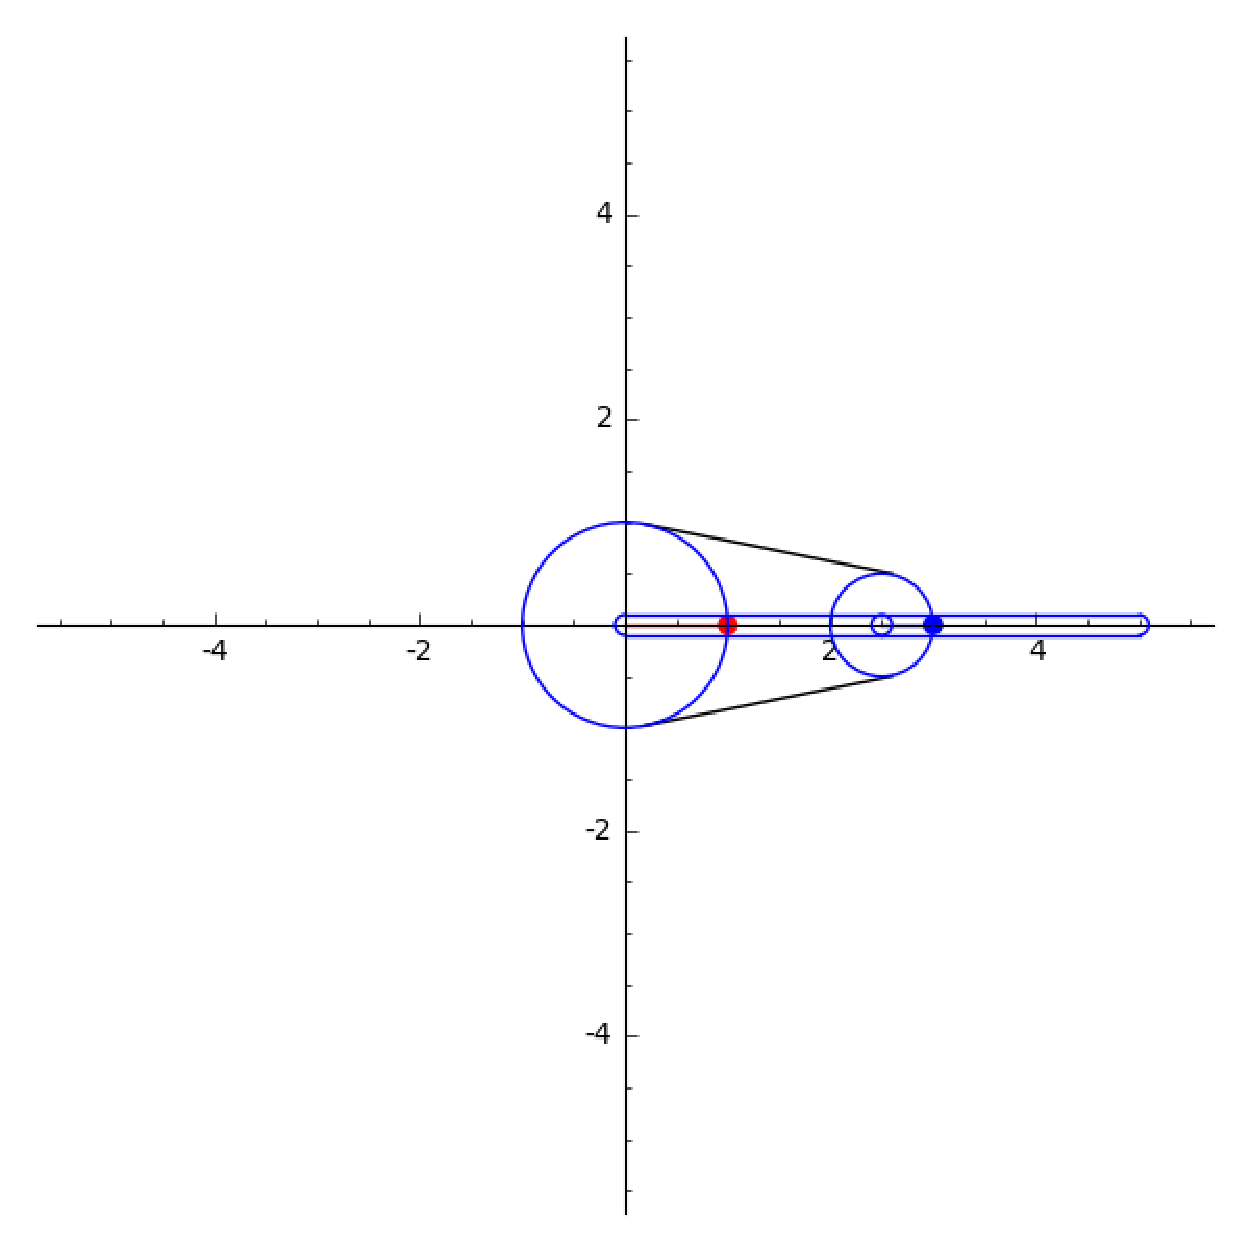
\includegraphics[width=0.3\columnwidth]{tri1.eps}
%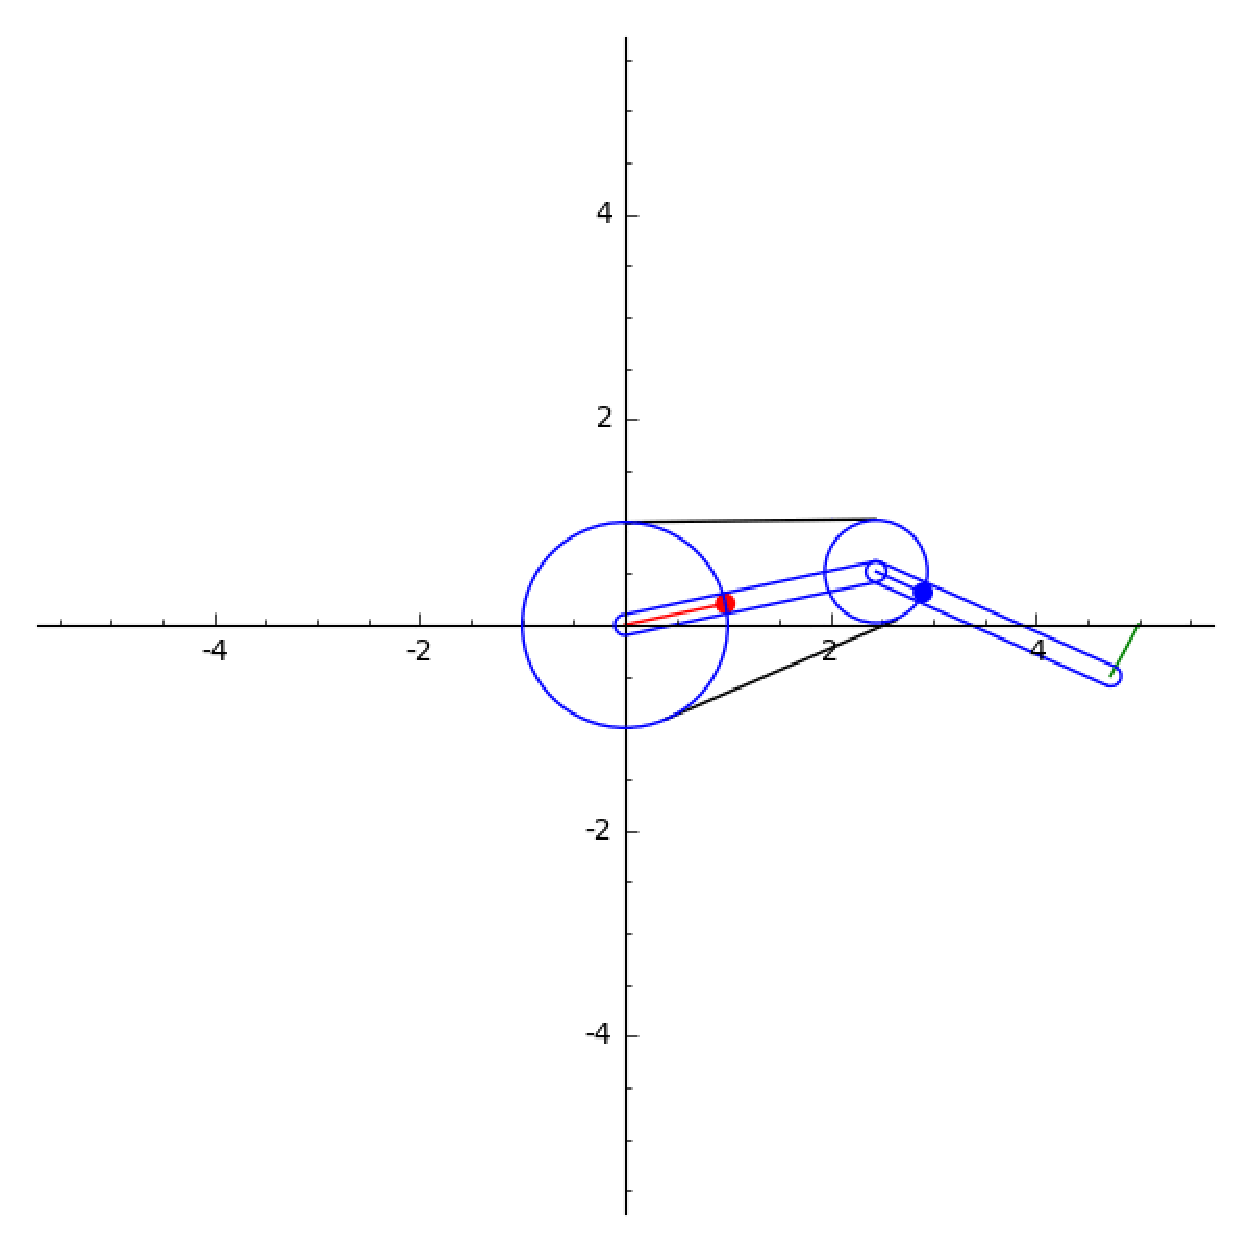
\includegraphics[width=0.3\columnwidth]{tri2.eps}
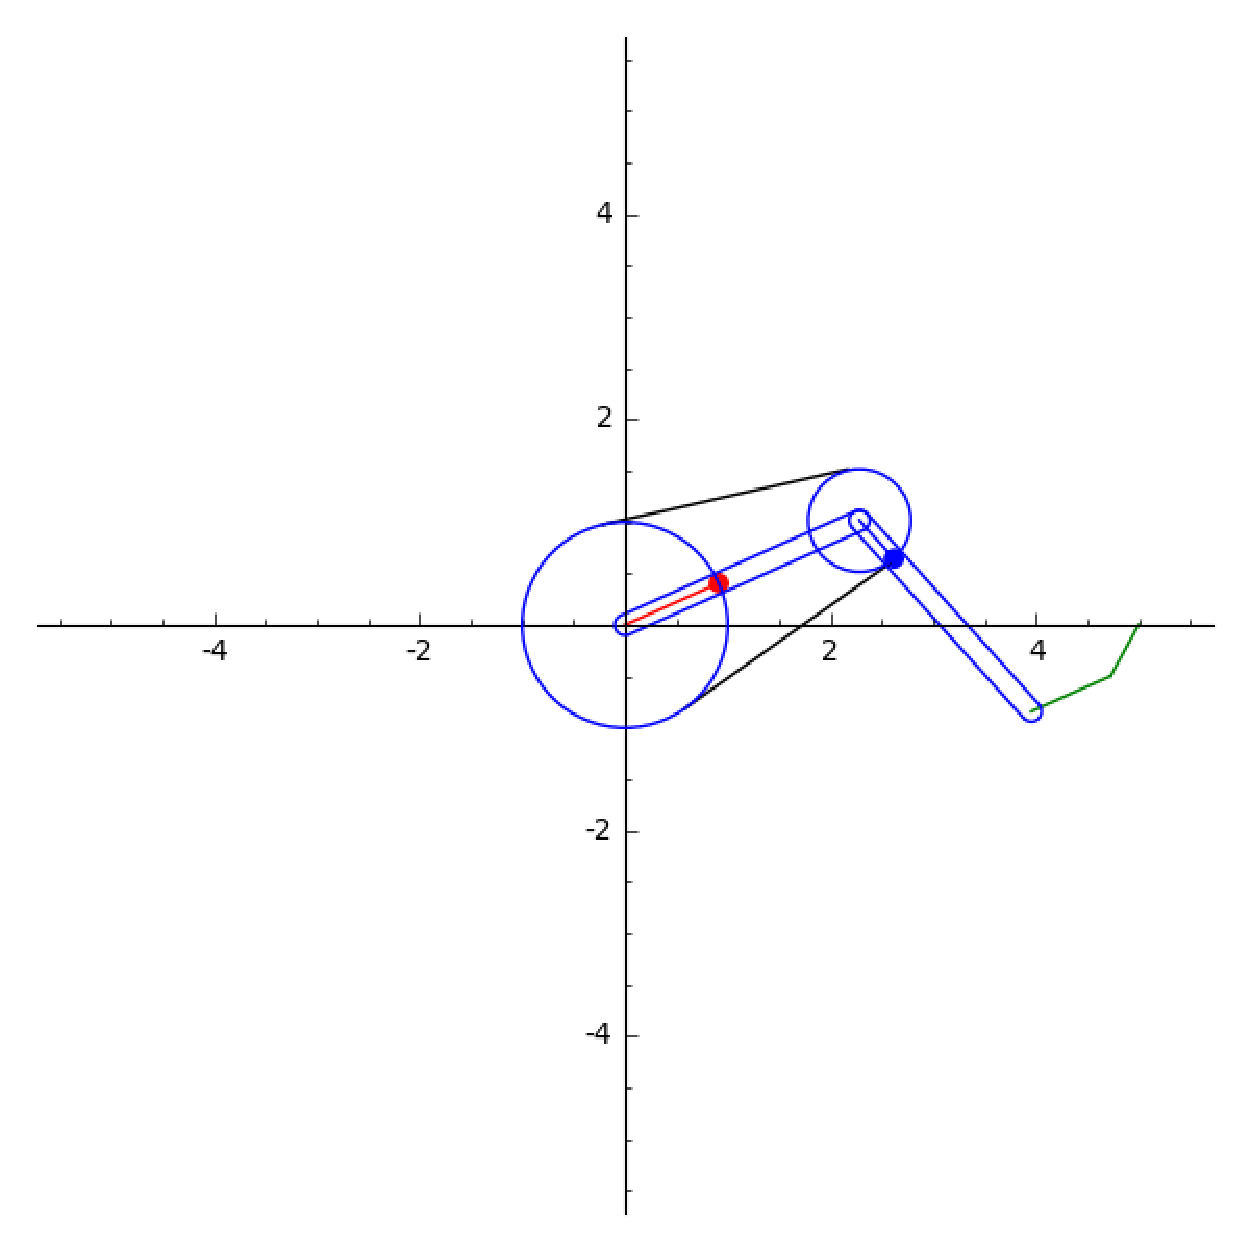
\includegraphics[width=0.3\columnwidth]{tri3.eps}
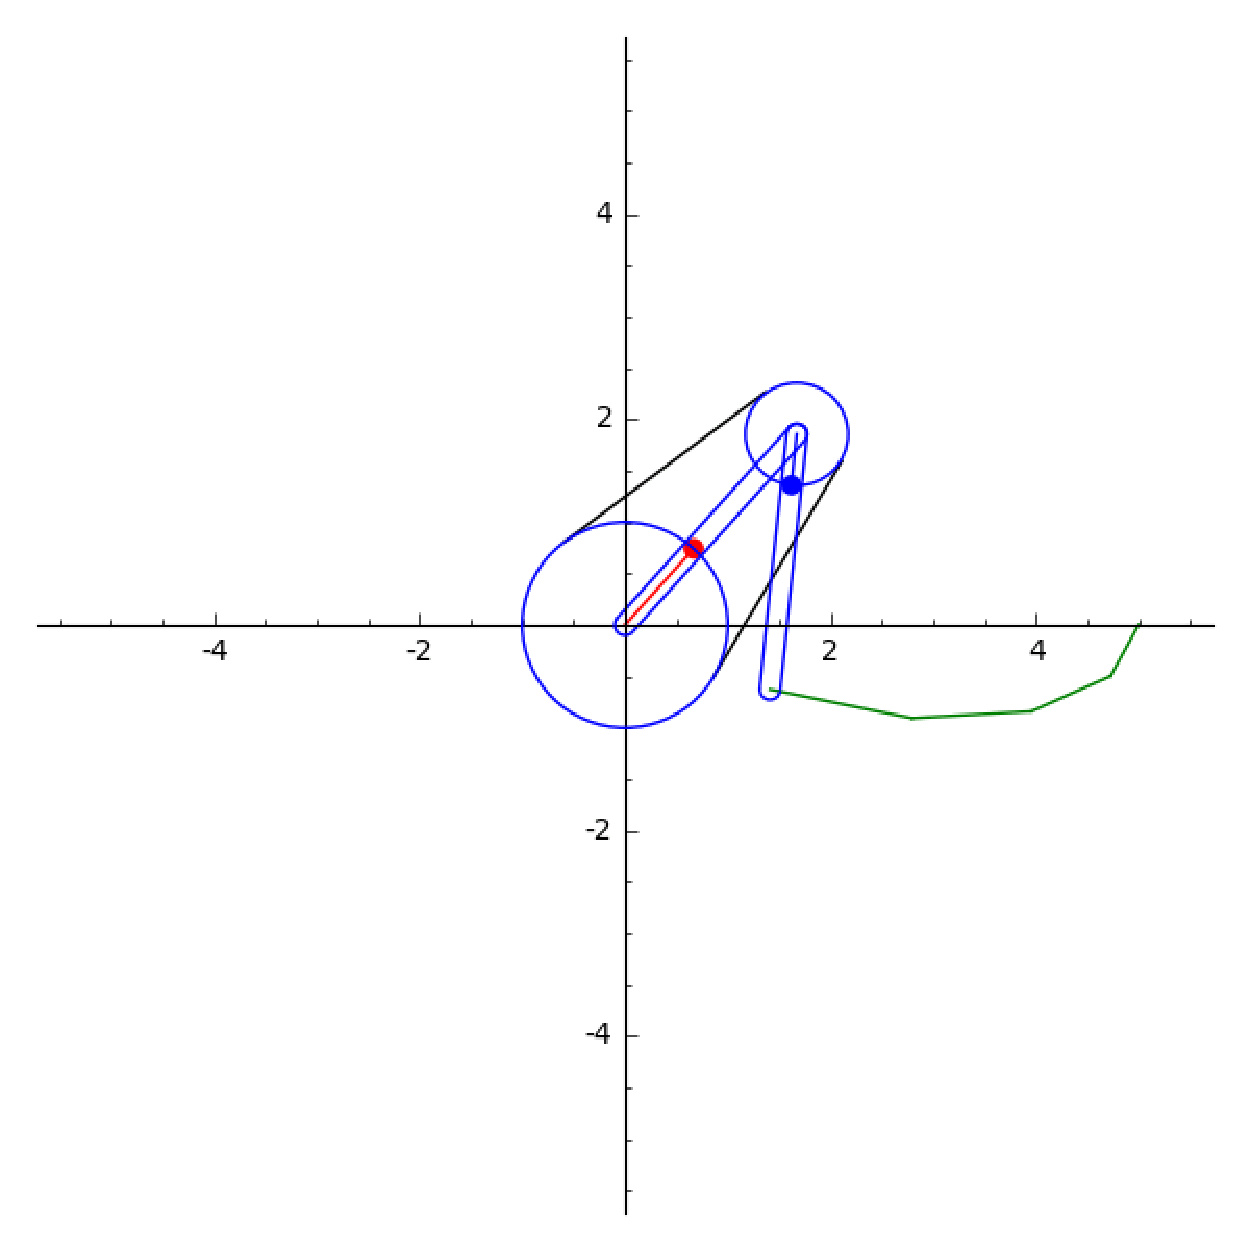
\includegraphics[width=0.3\columnwidth]{tri5.eps}\\[1em]
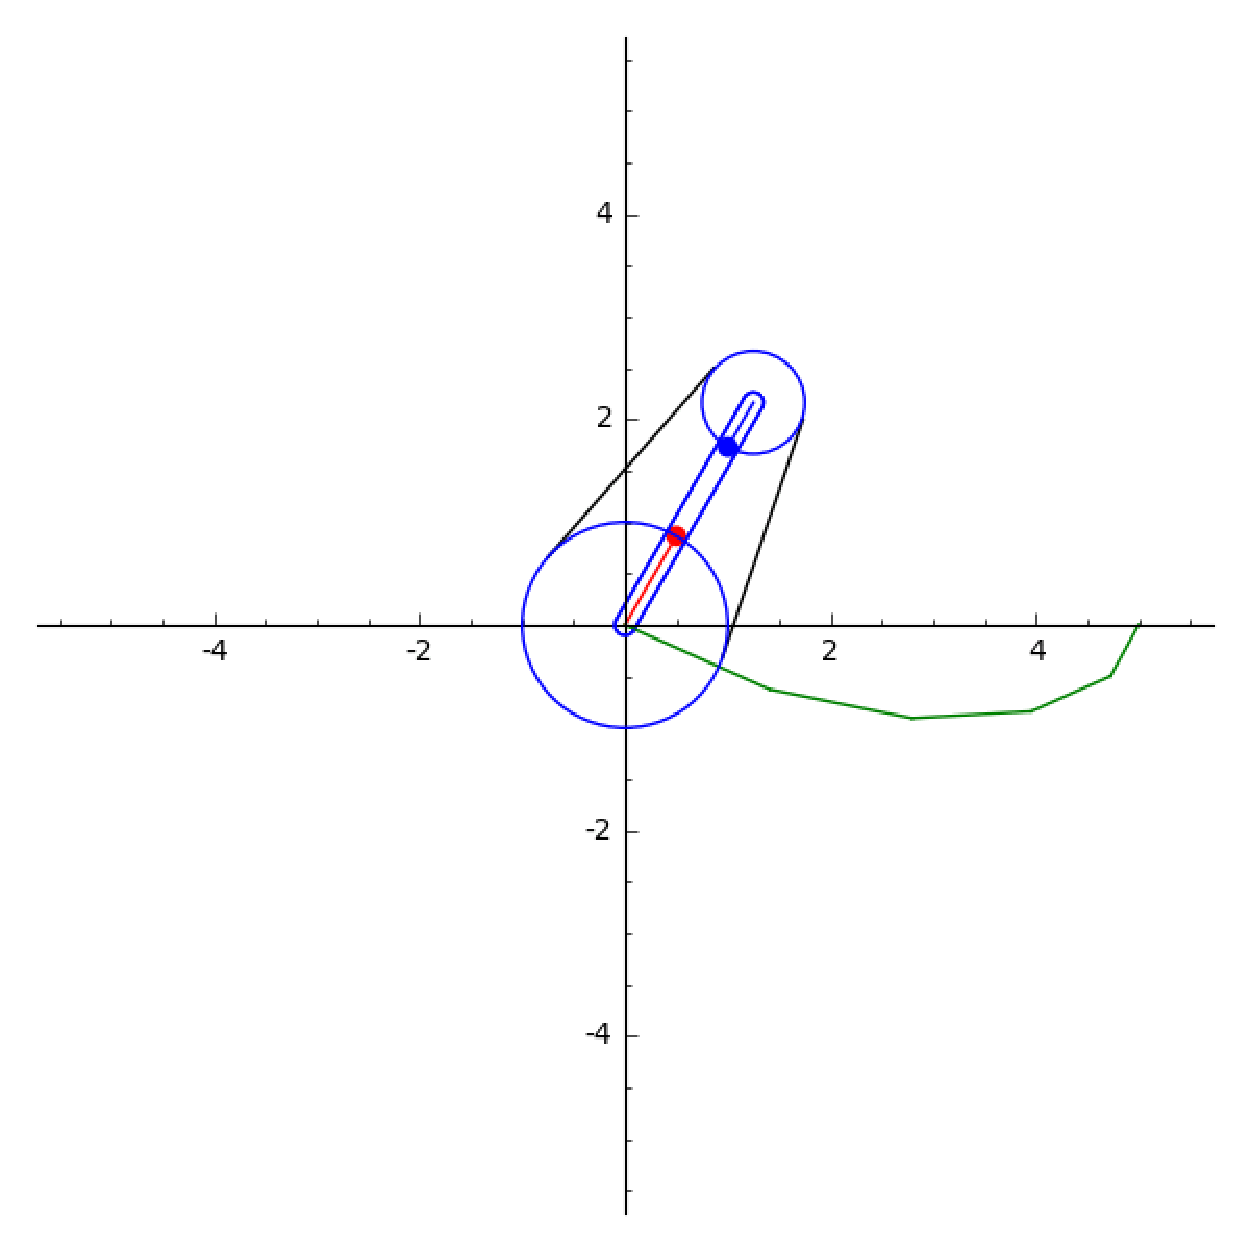
\includegraphics[width=0.3\columnwidth]{tri6.eps}
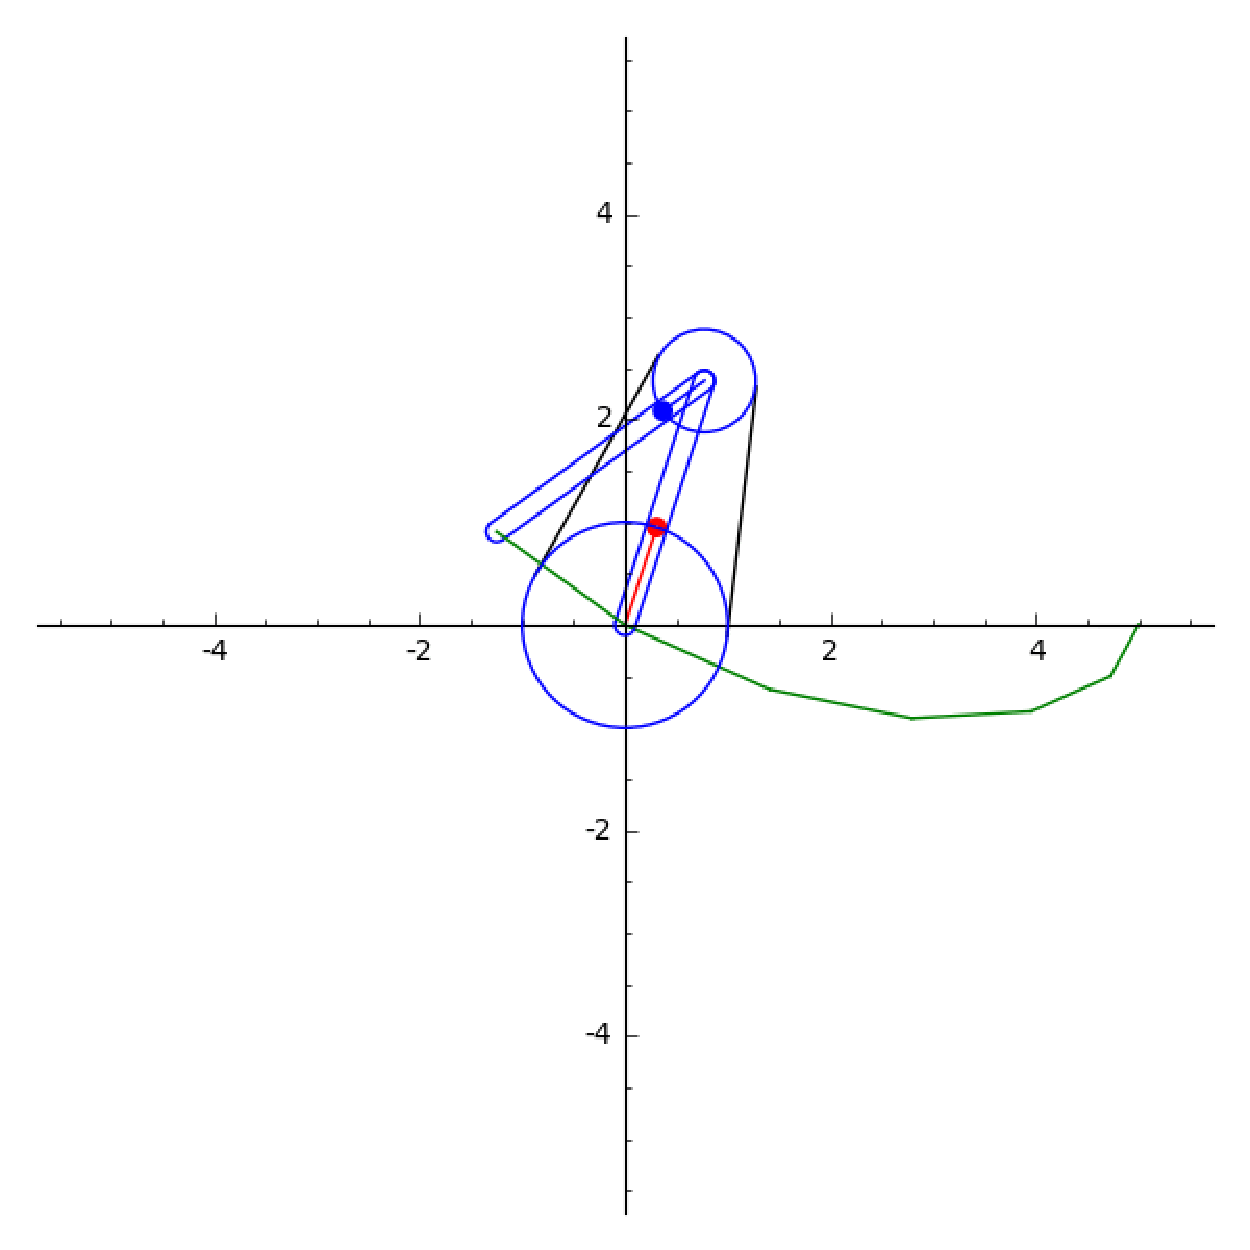
\includegraphics[width=0.3\columnwidth]{tri7.eps}
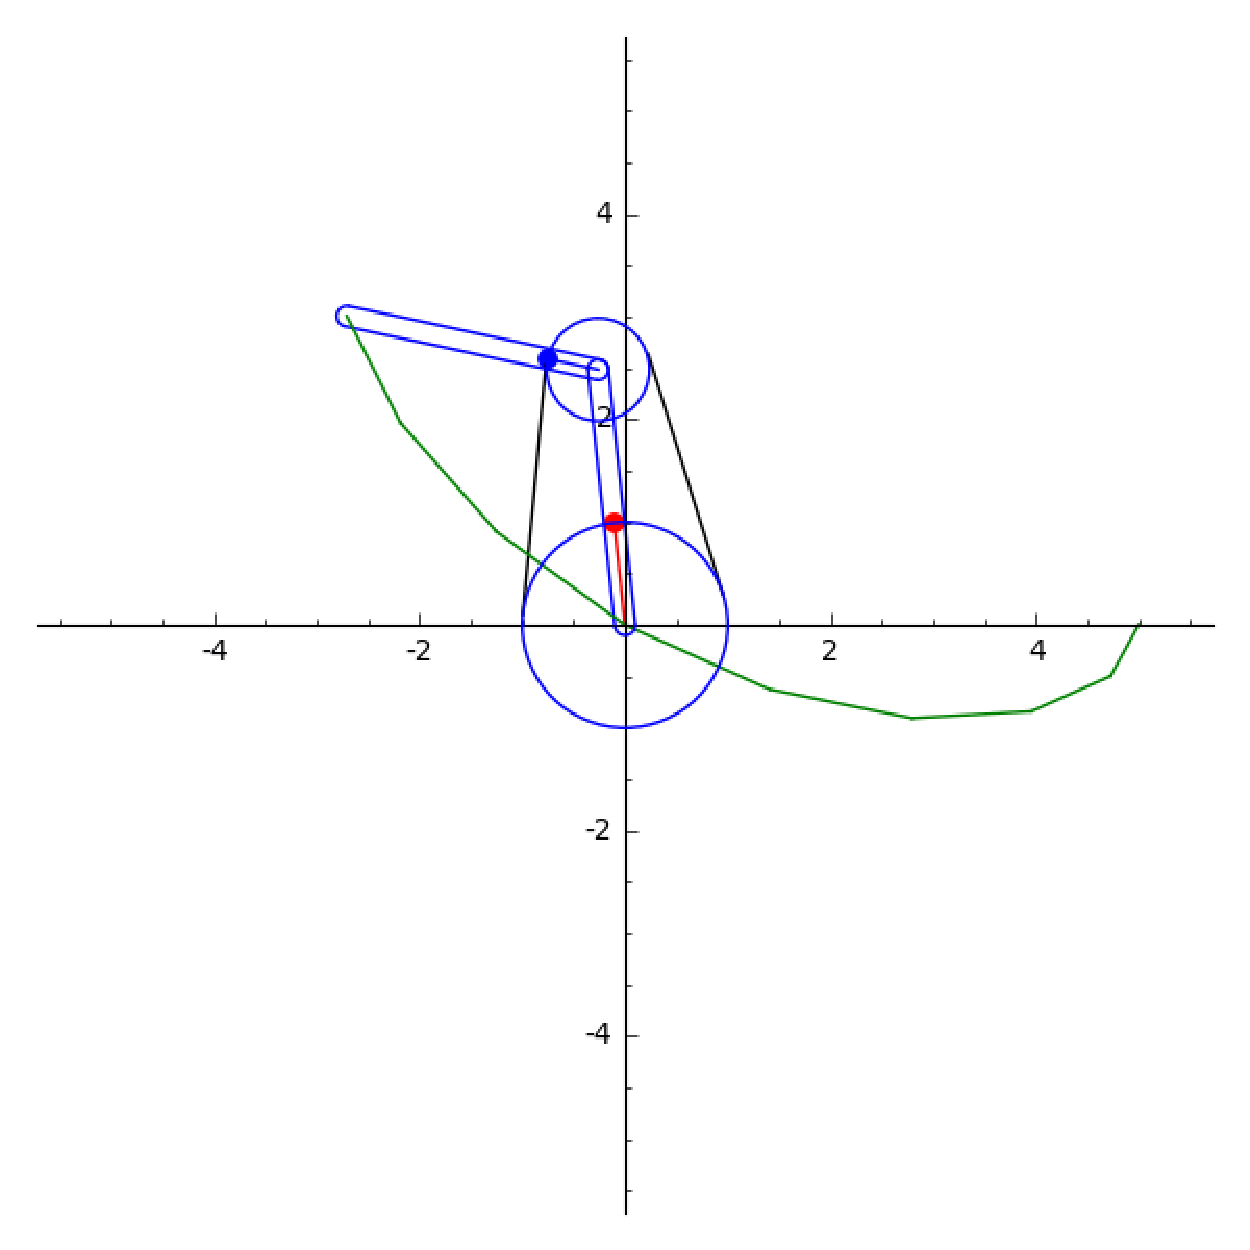
\includegraphics[width=0.3\columnwidth]{tri9.eps}\\[1em]
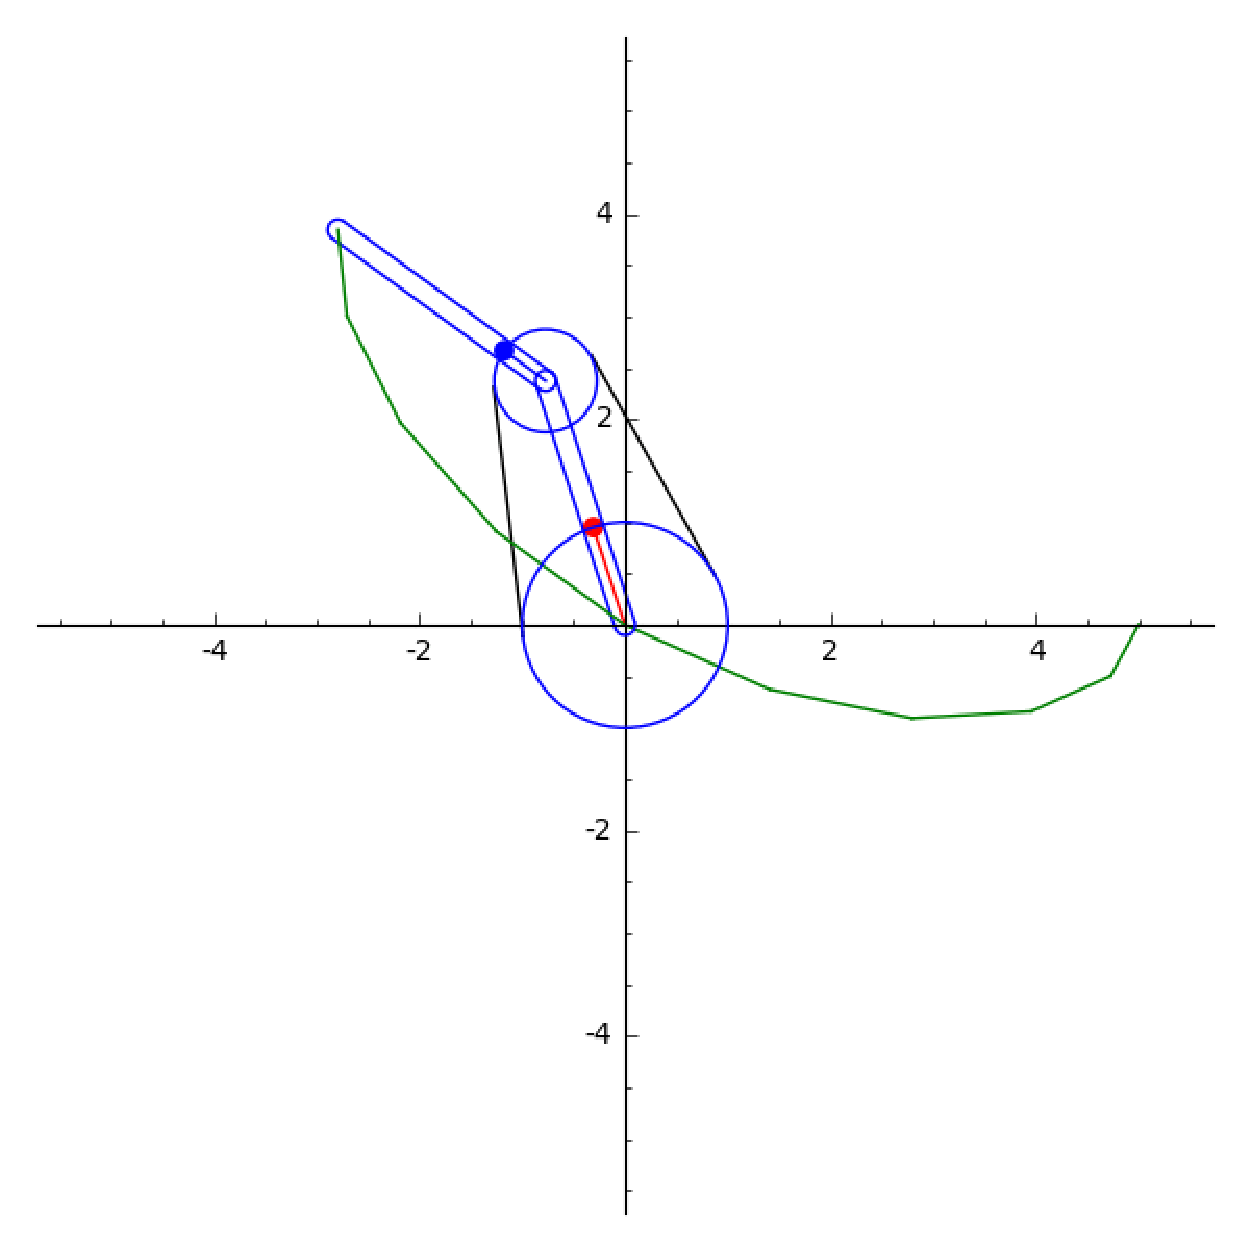
\includegraphics[width=0.3\columnwidth]{tri10.eps}
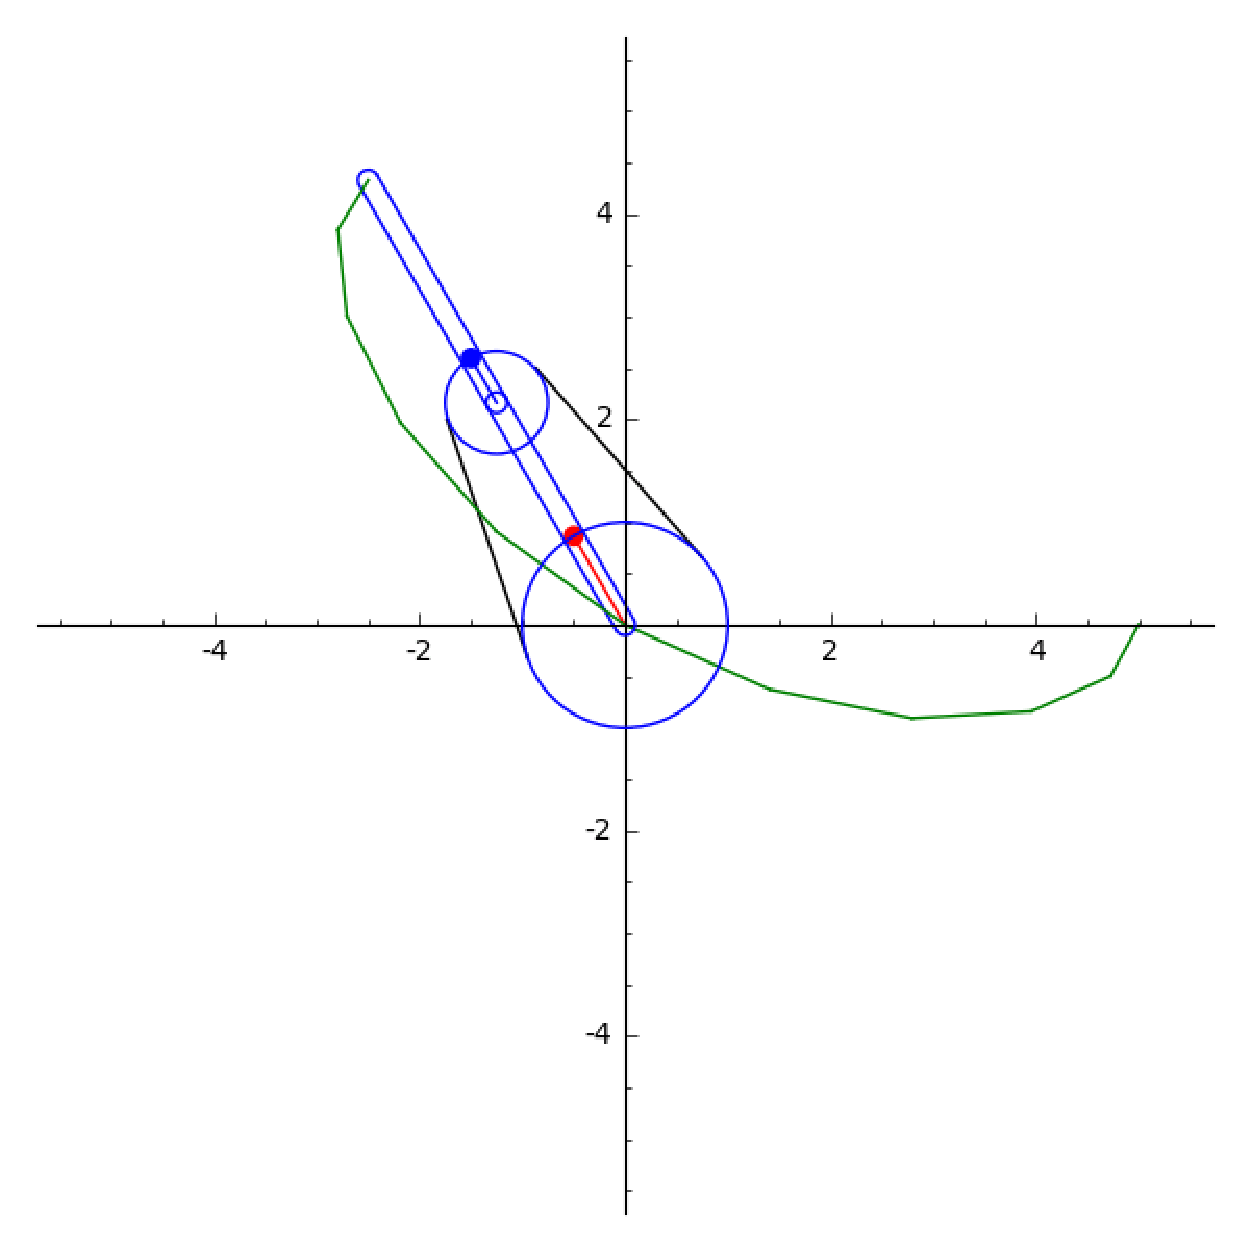
\includegraphics[width=0.3\columnwidth]{tri11.eps}
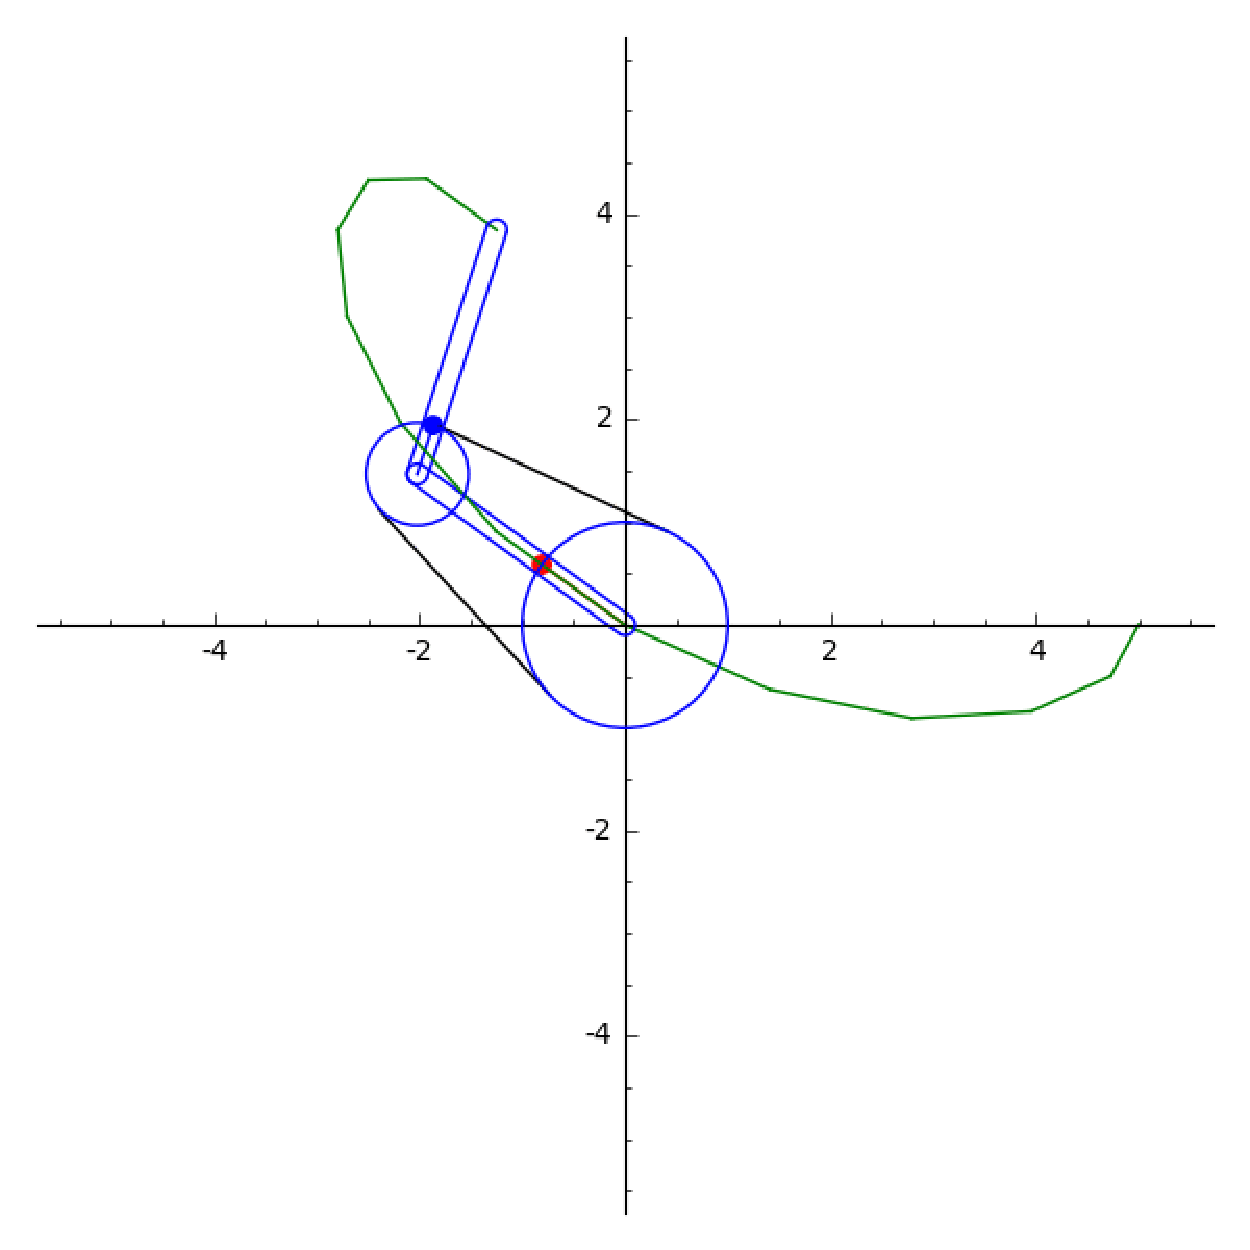
\includegraphics[width=0.3\columnwidth]{tri13.eps}\\[1em]
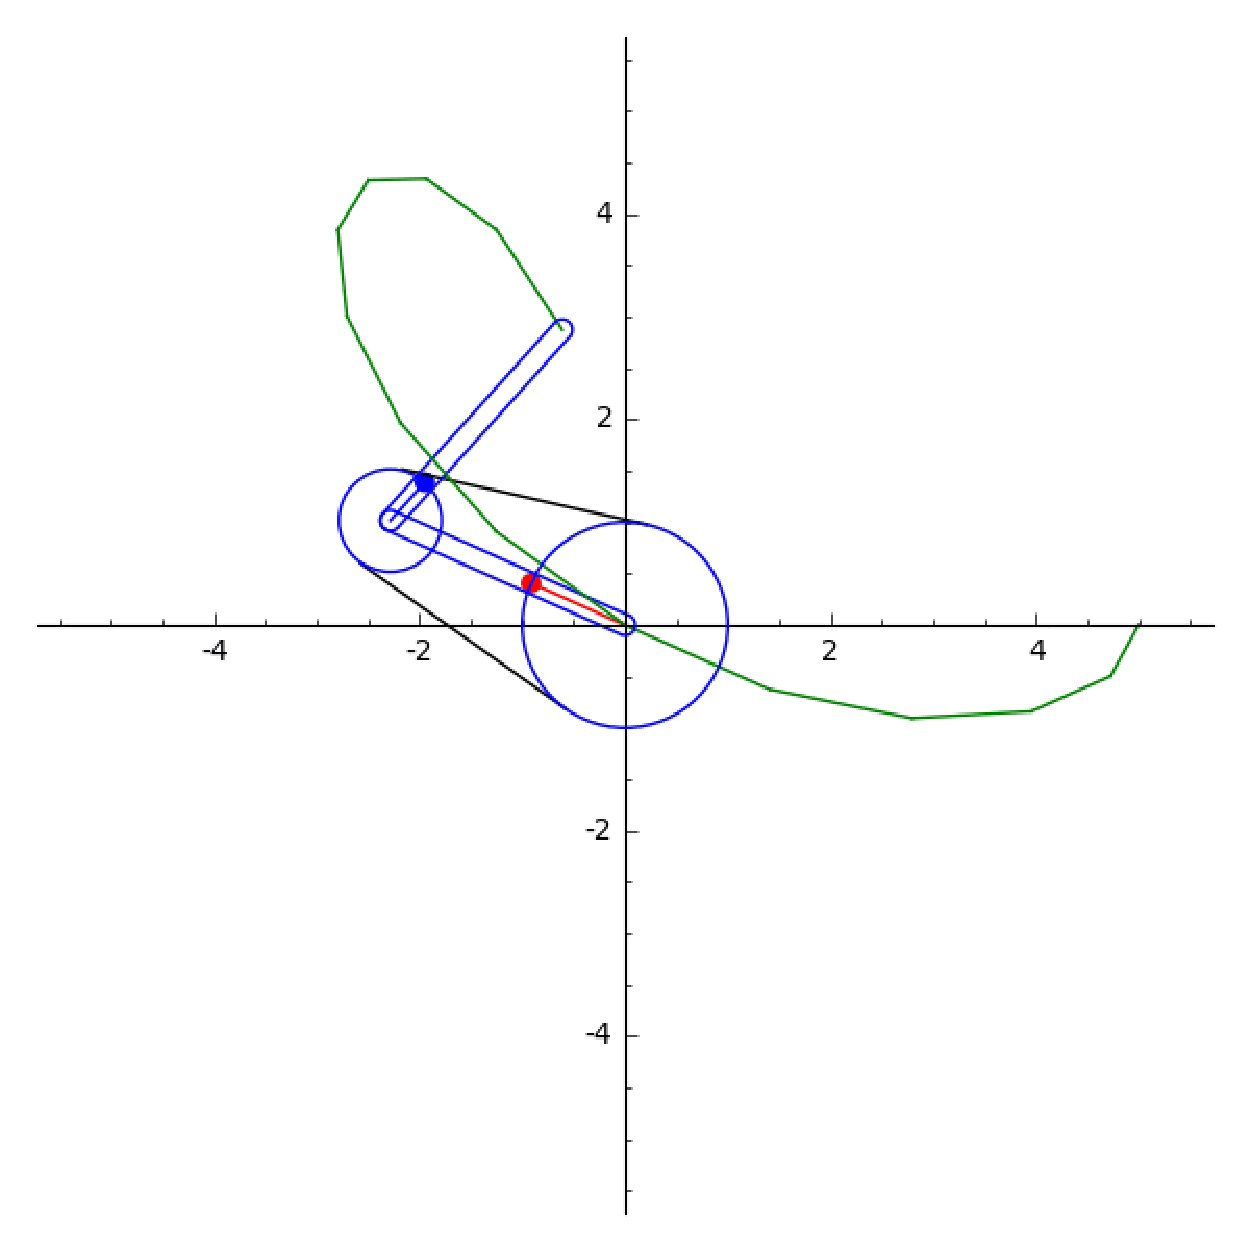
\includegraphics[width=0.3\columnwidth]{tri14.eps}
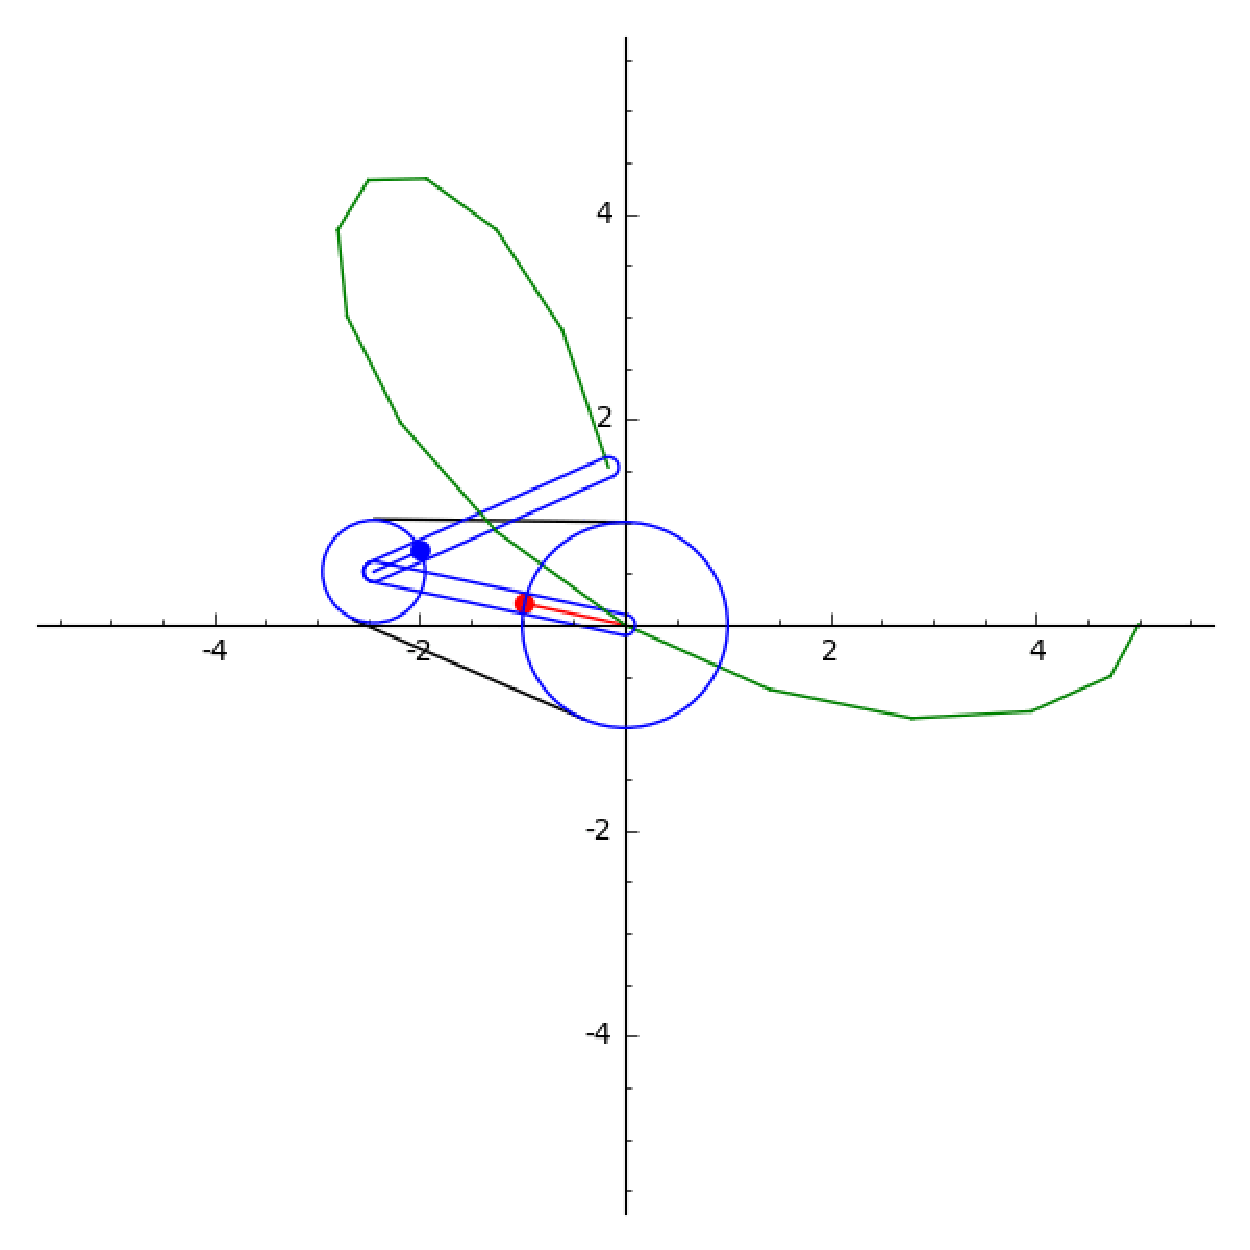
\includegraphics[width=0.3\columnwidth]{tri15.eps}
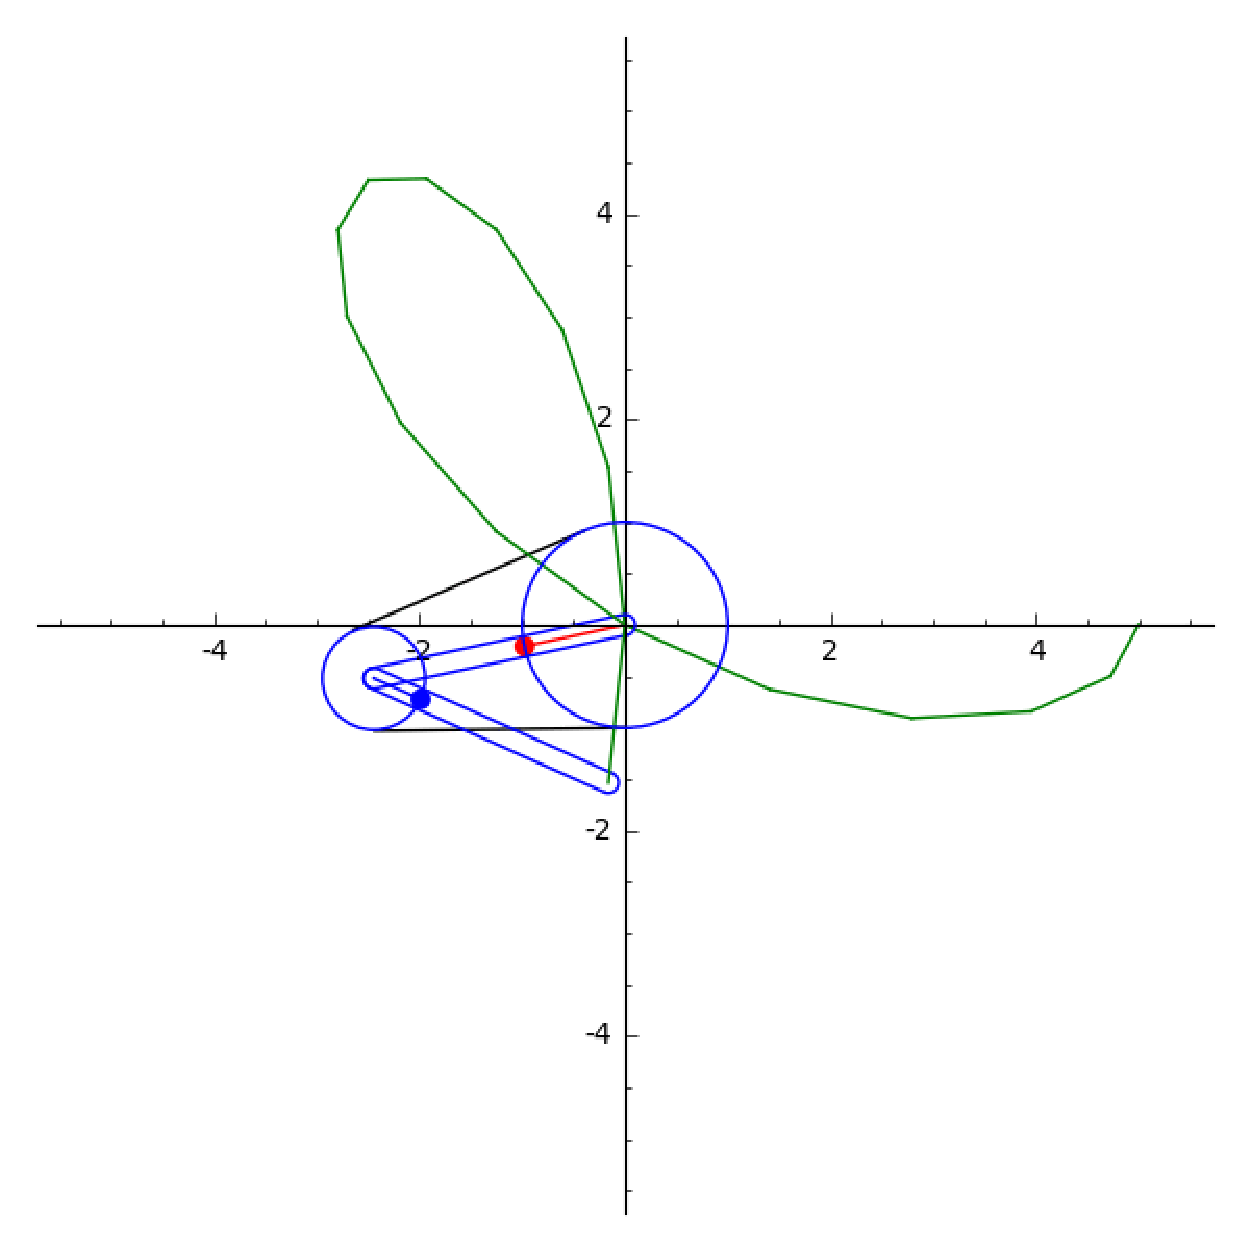
\includegraphics[width=0.3\columnwidth]{tri17.eps}\\[1em]
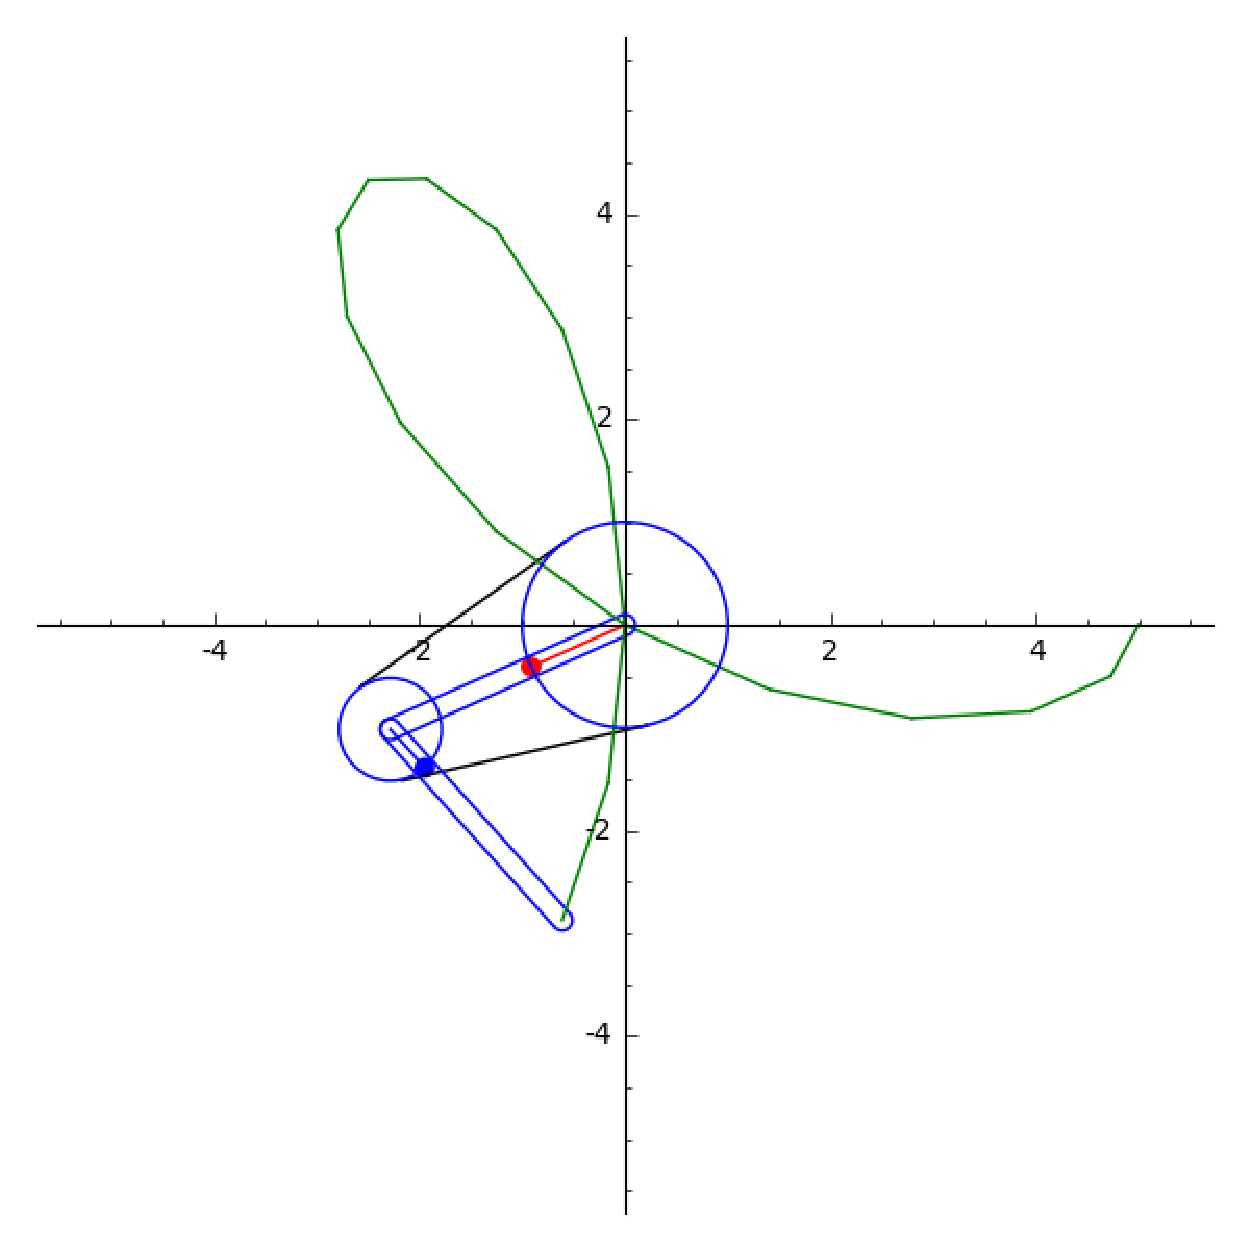
\includegraphics[width=0.3\columnwidth]{tri18.eps}
%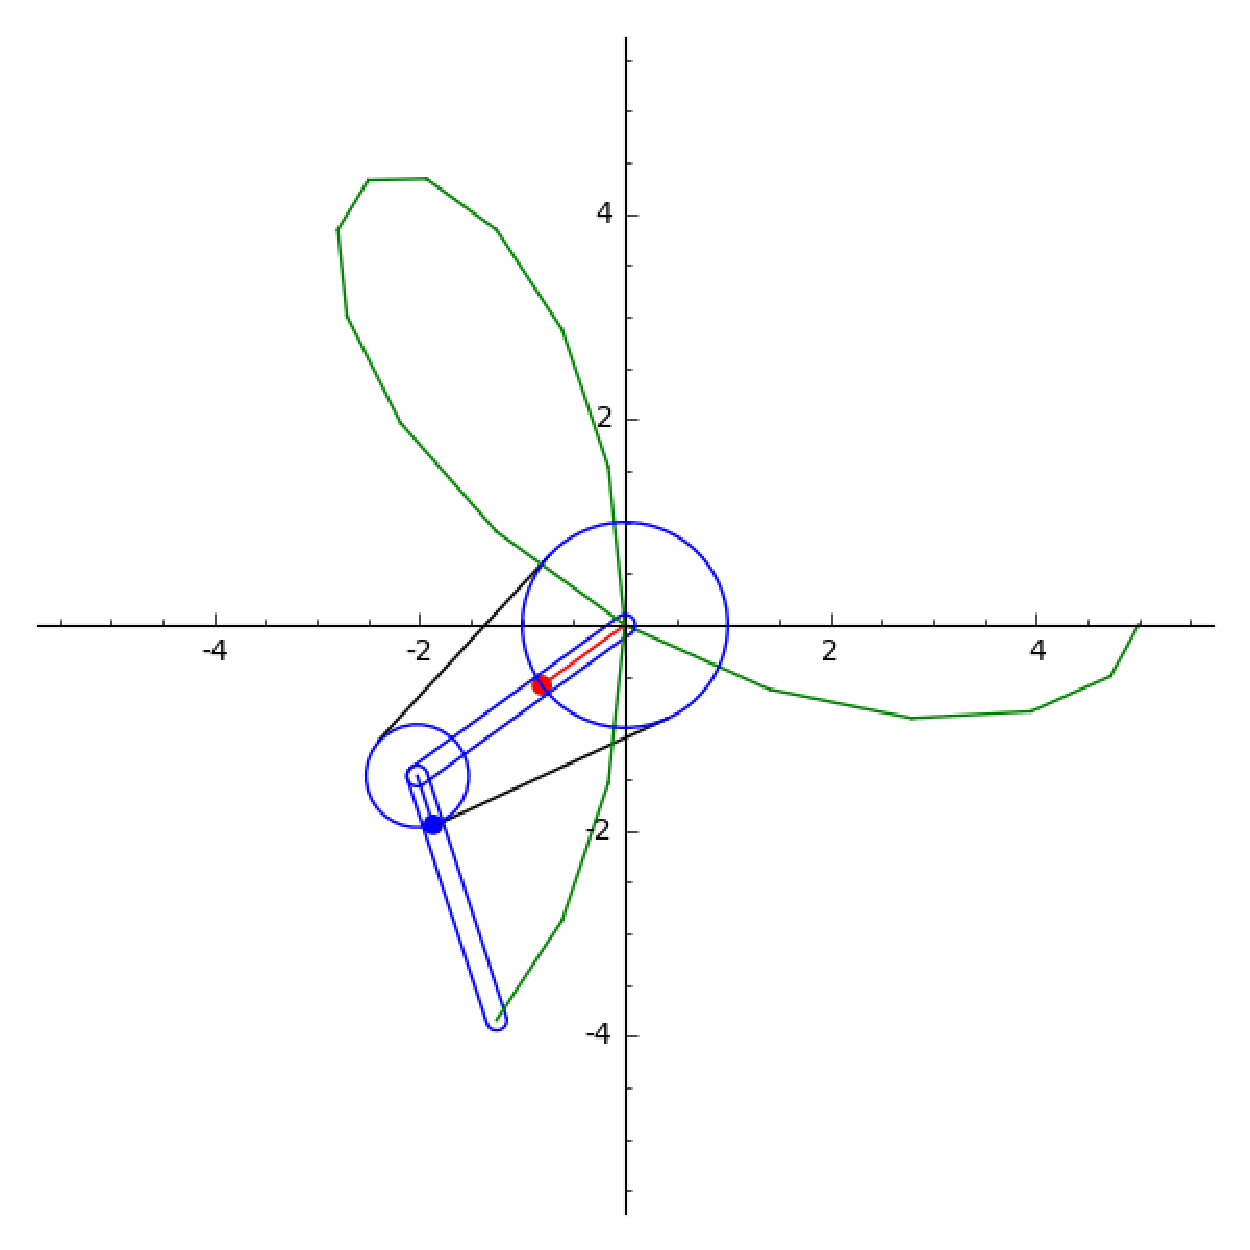
\includegraphics[width=0.3\columnwidth]{tri19.eps}
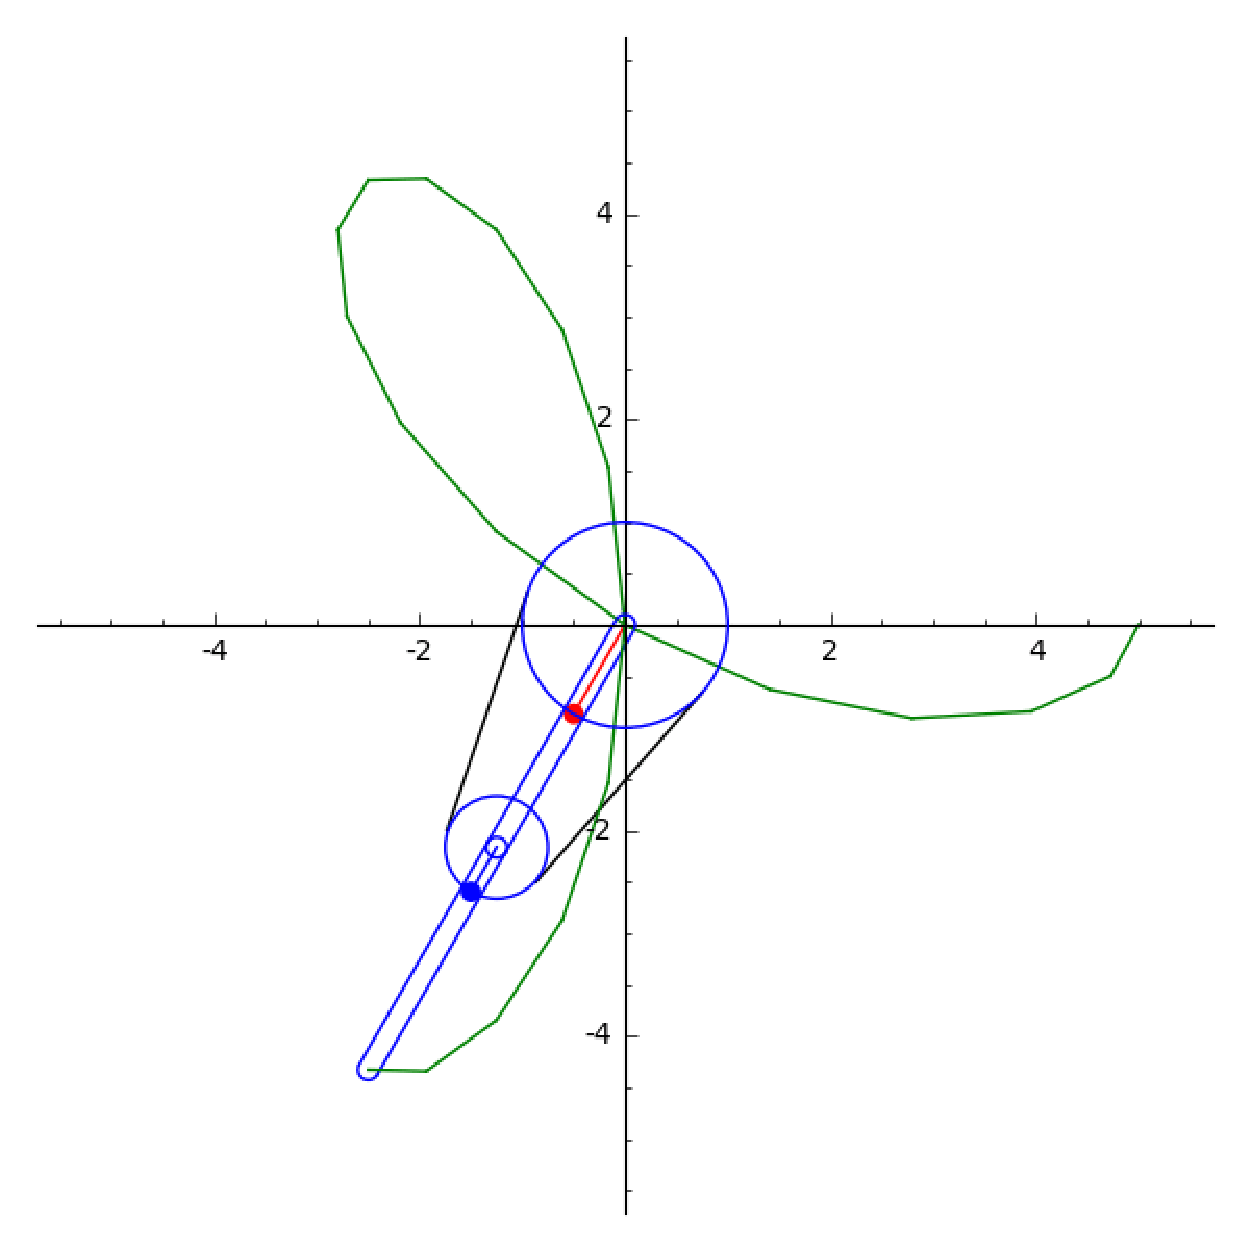
\includegraphics[width=0.3\columnwidth]{tri21.eps}
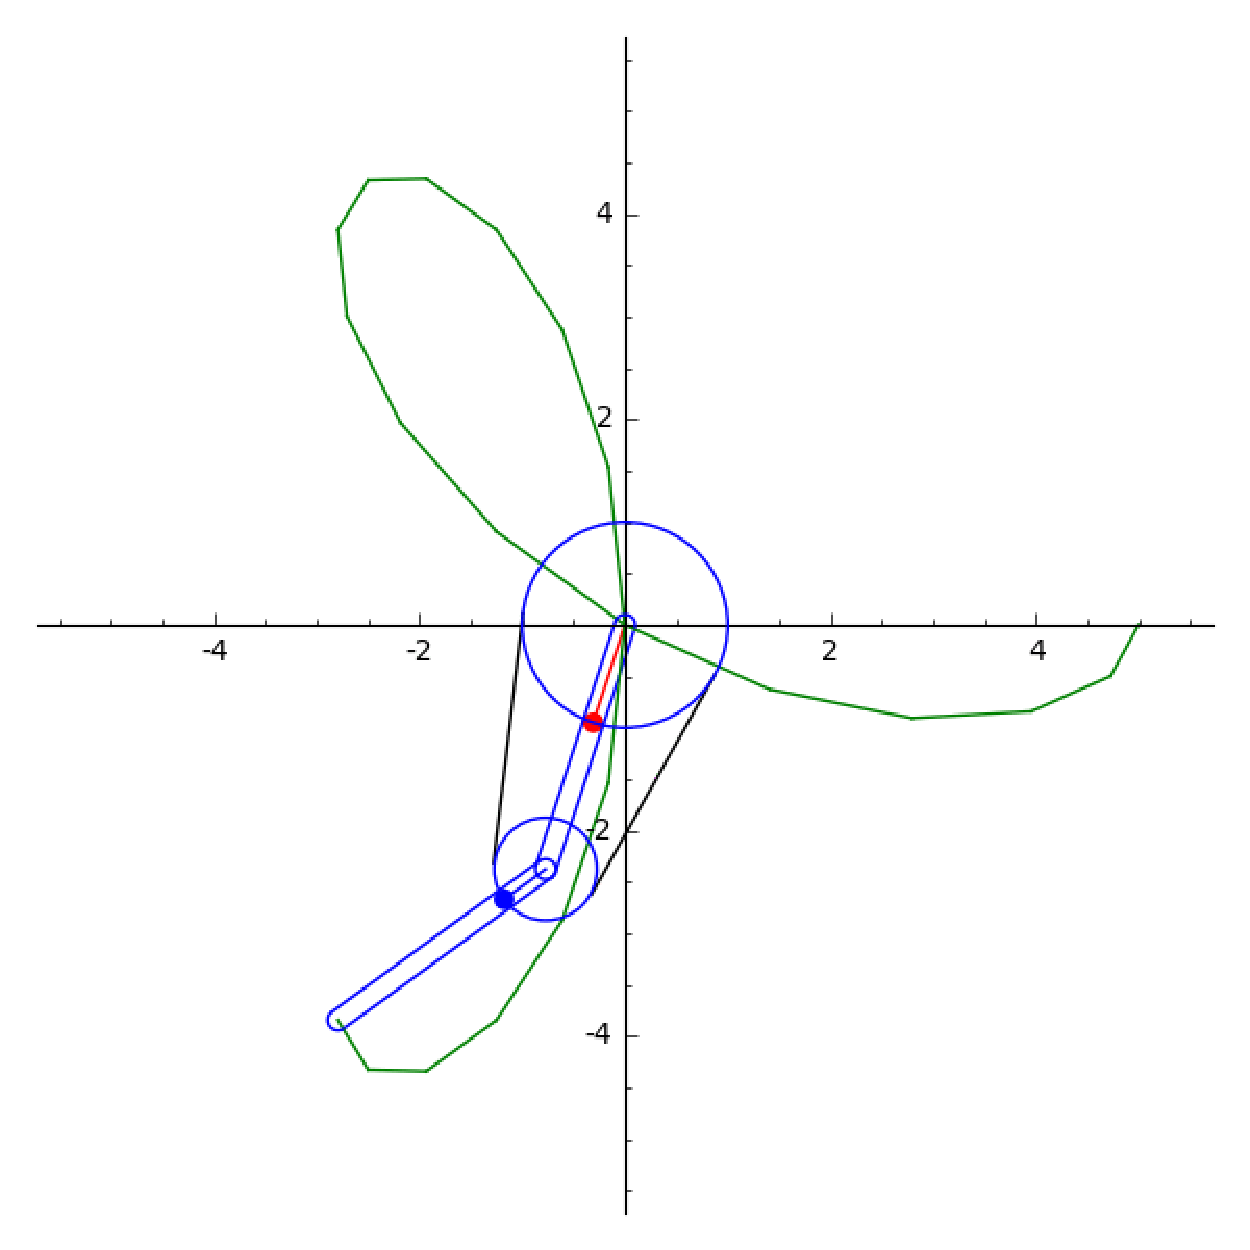
\includegraphics[width=0.3\columnwidth]{tri22.eps}\\[1em]
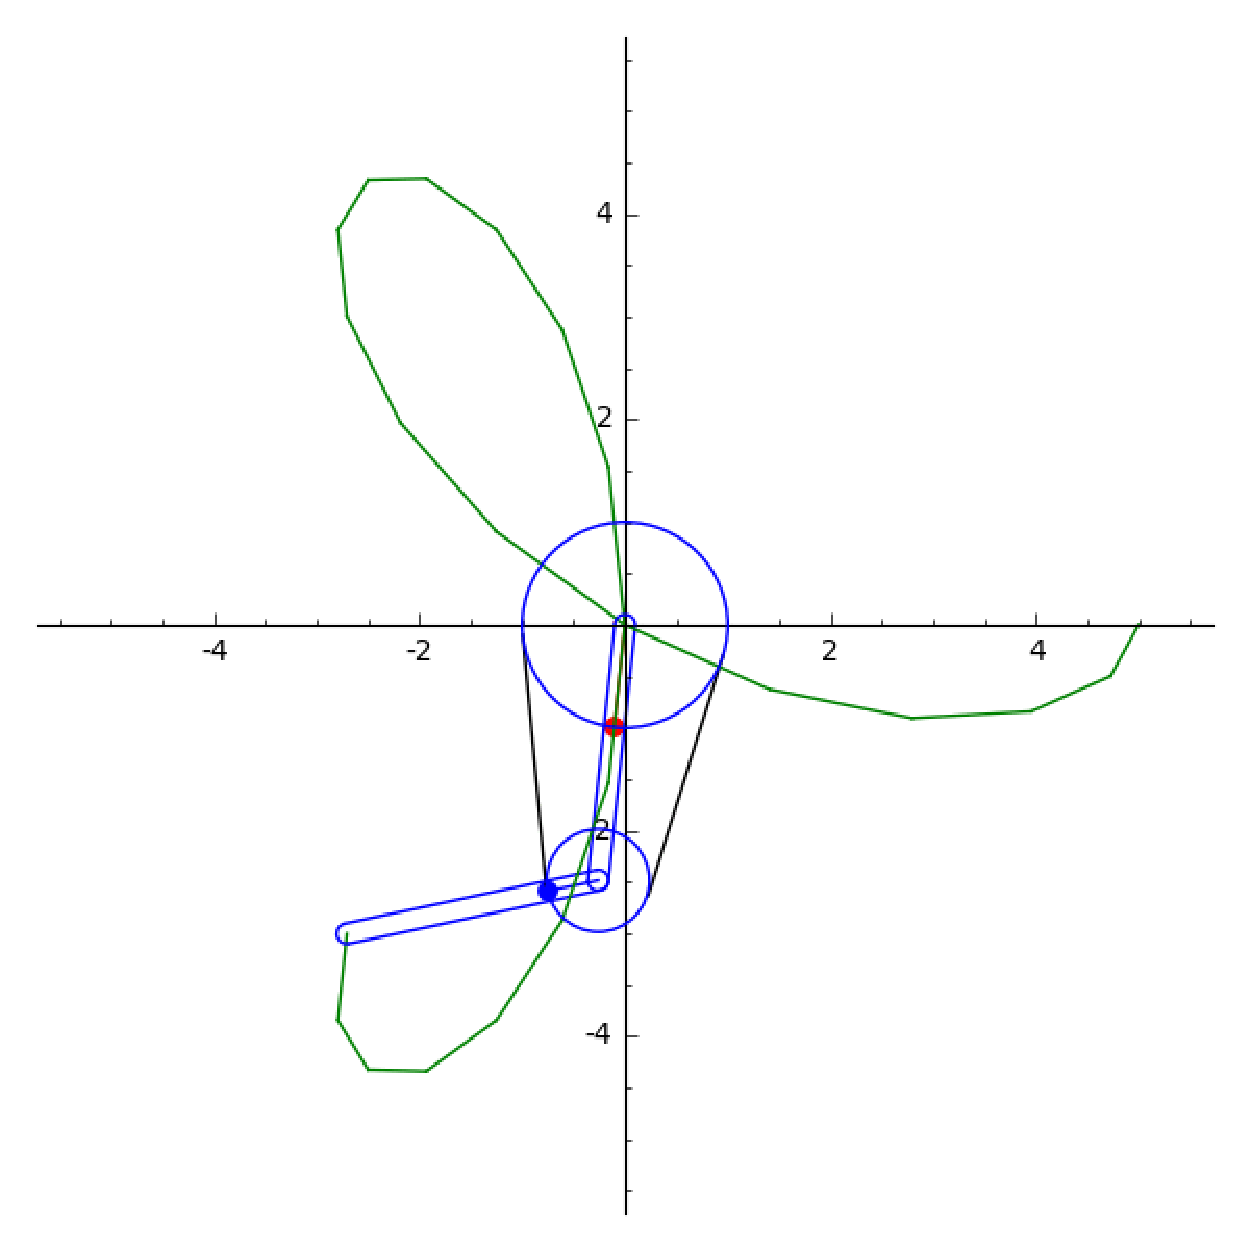
\includegraphics[width=0.3\columnwidth]{tri23.eps}
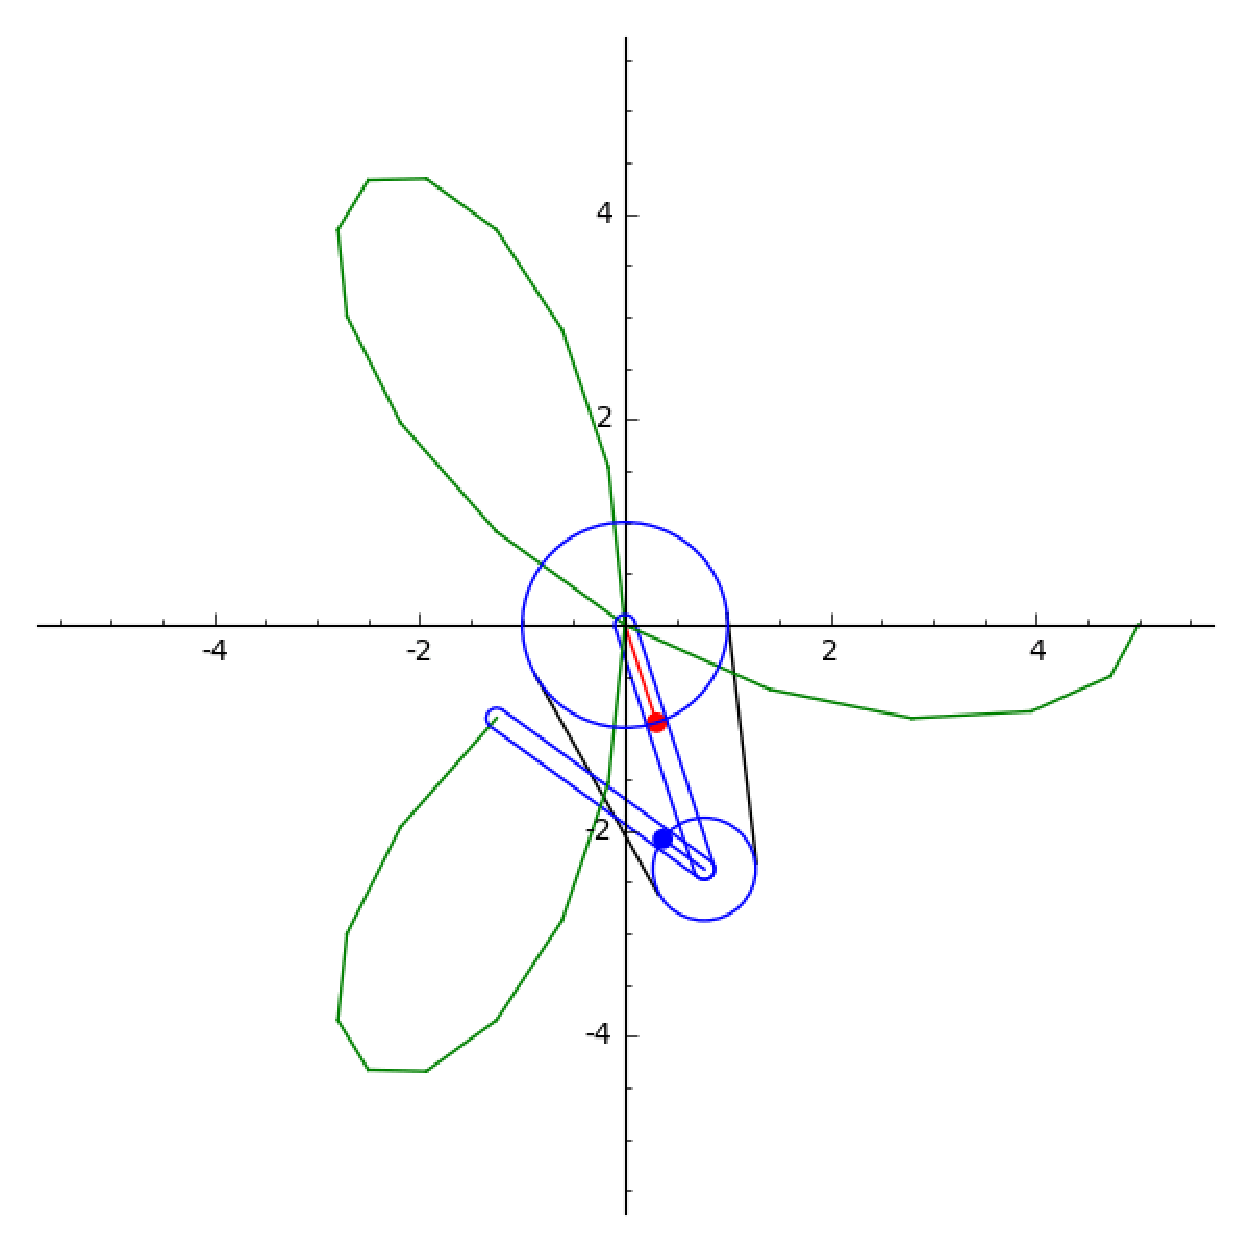
\includegraphics[width=0.3\columnwidth]{tri25.eps}
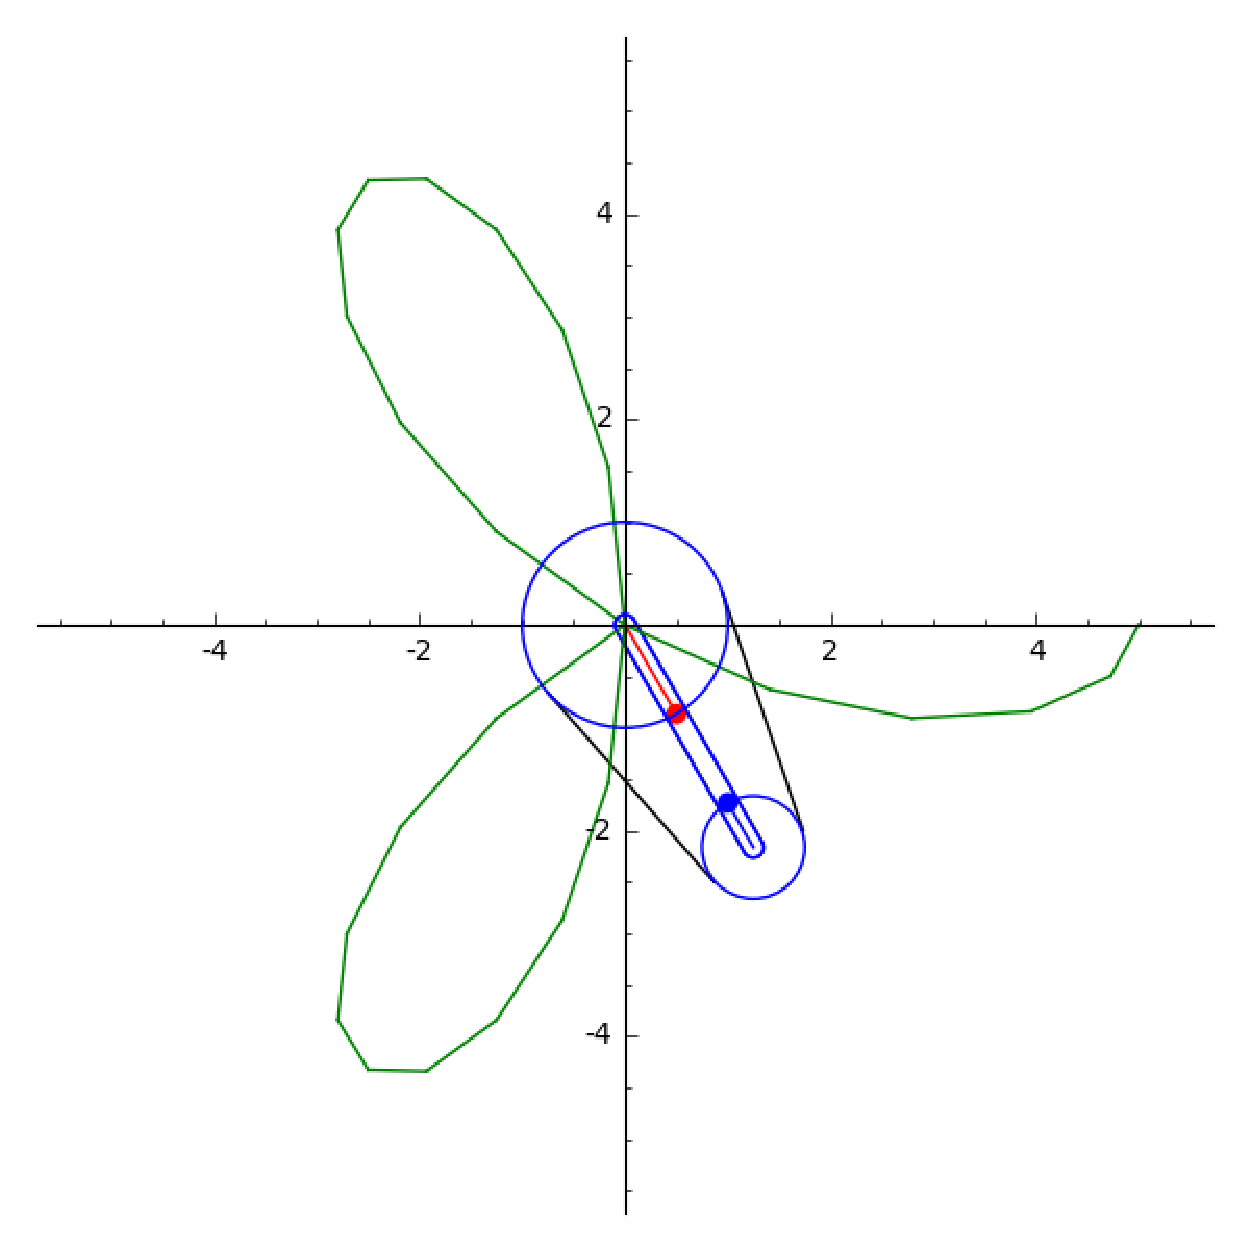
\includegraphics[width=0.3\columnwidth]{tri26.eps}\\[1em]
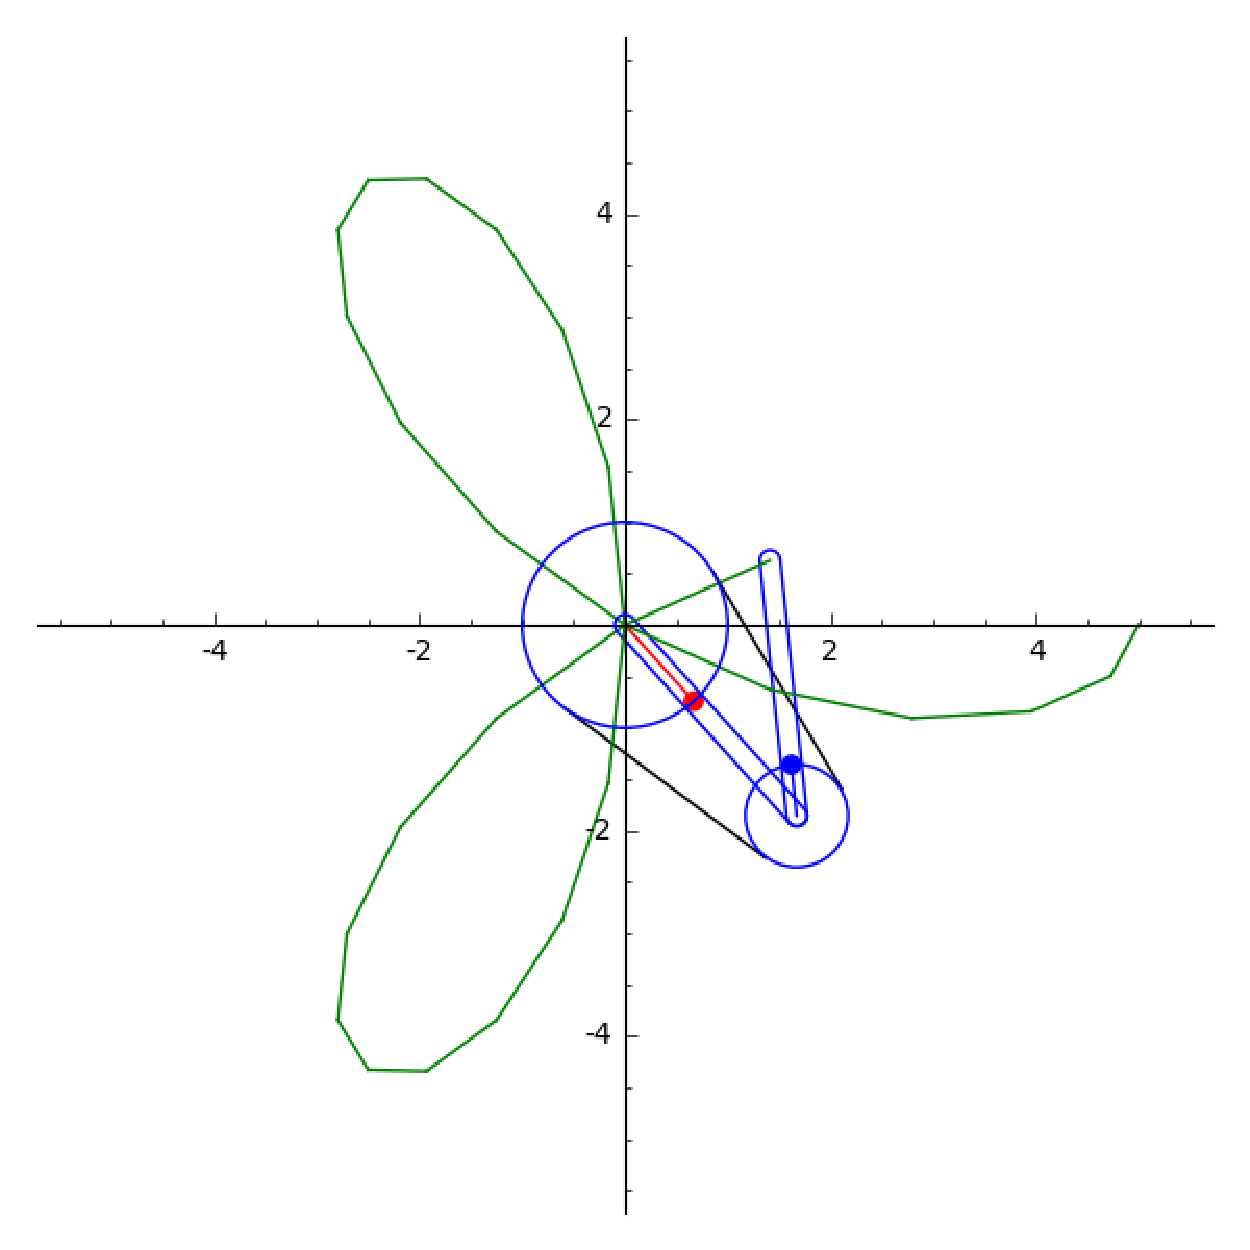
\includegraphics[width=0.3\columnwidth]{tri27.eps}
%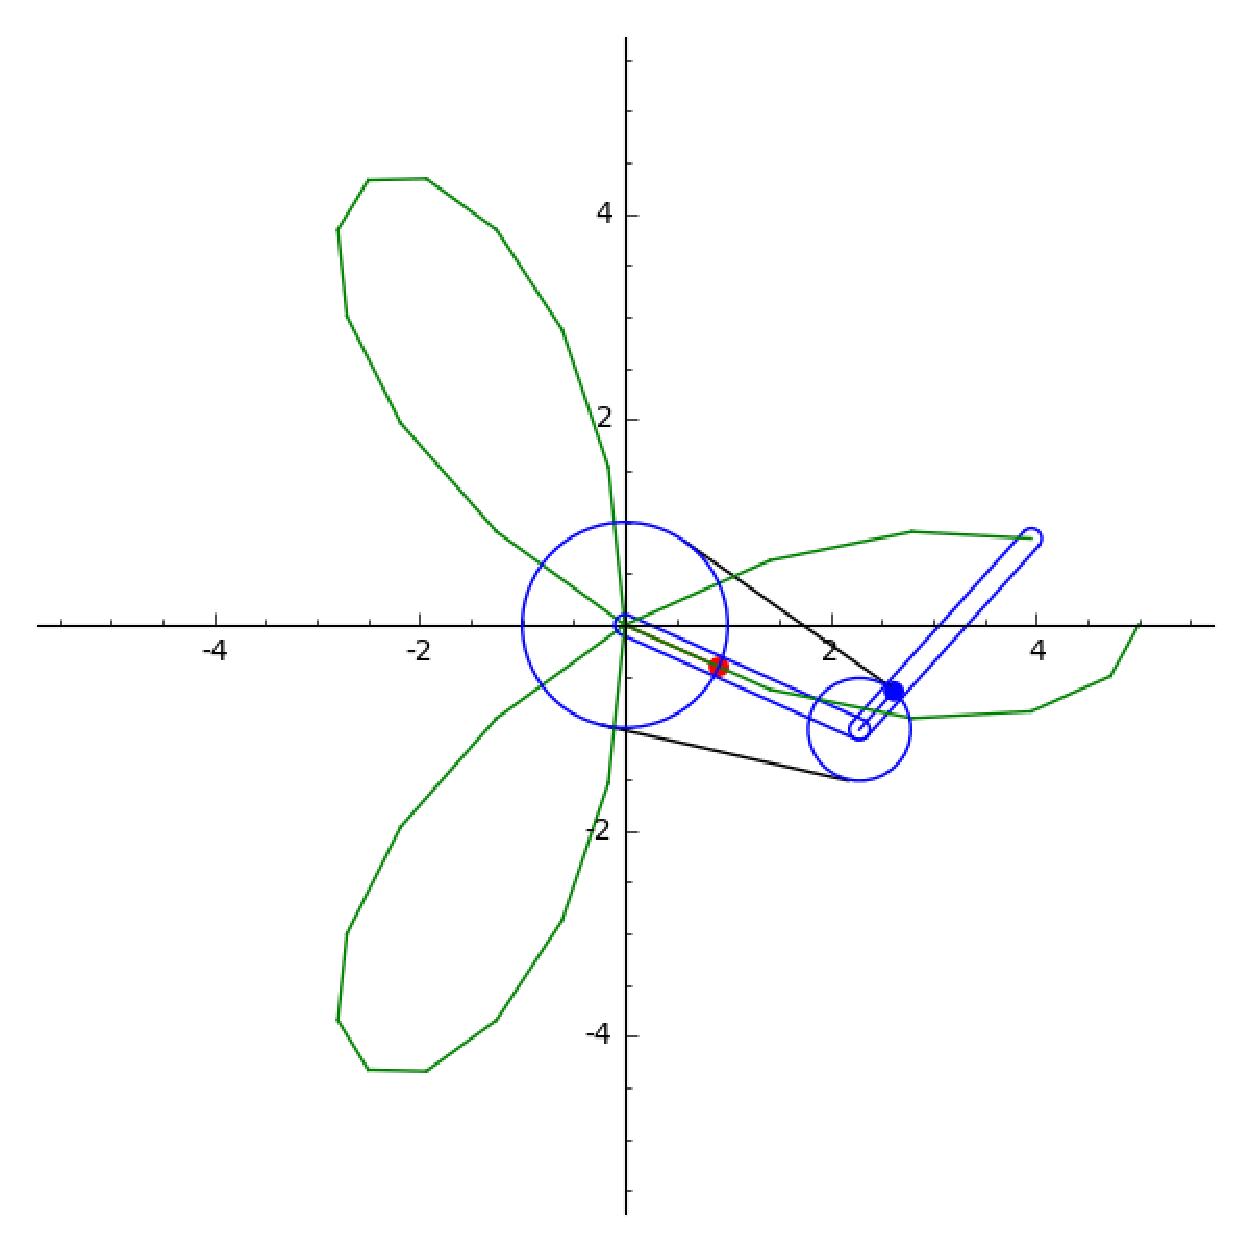
\includegraphics[width=0.3\columnwidth]{tri29.eps}
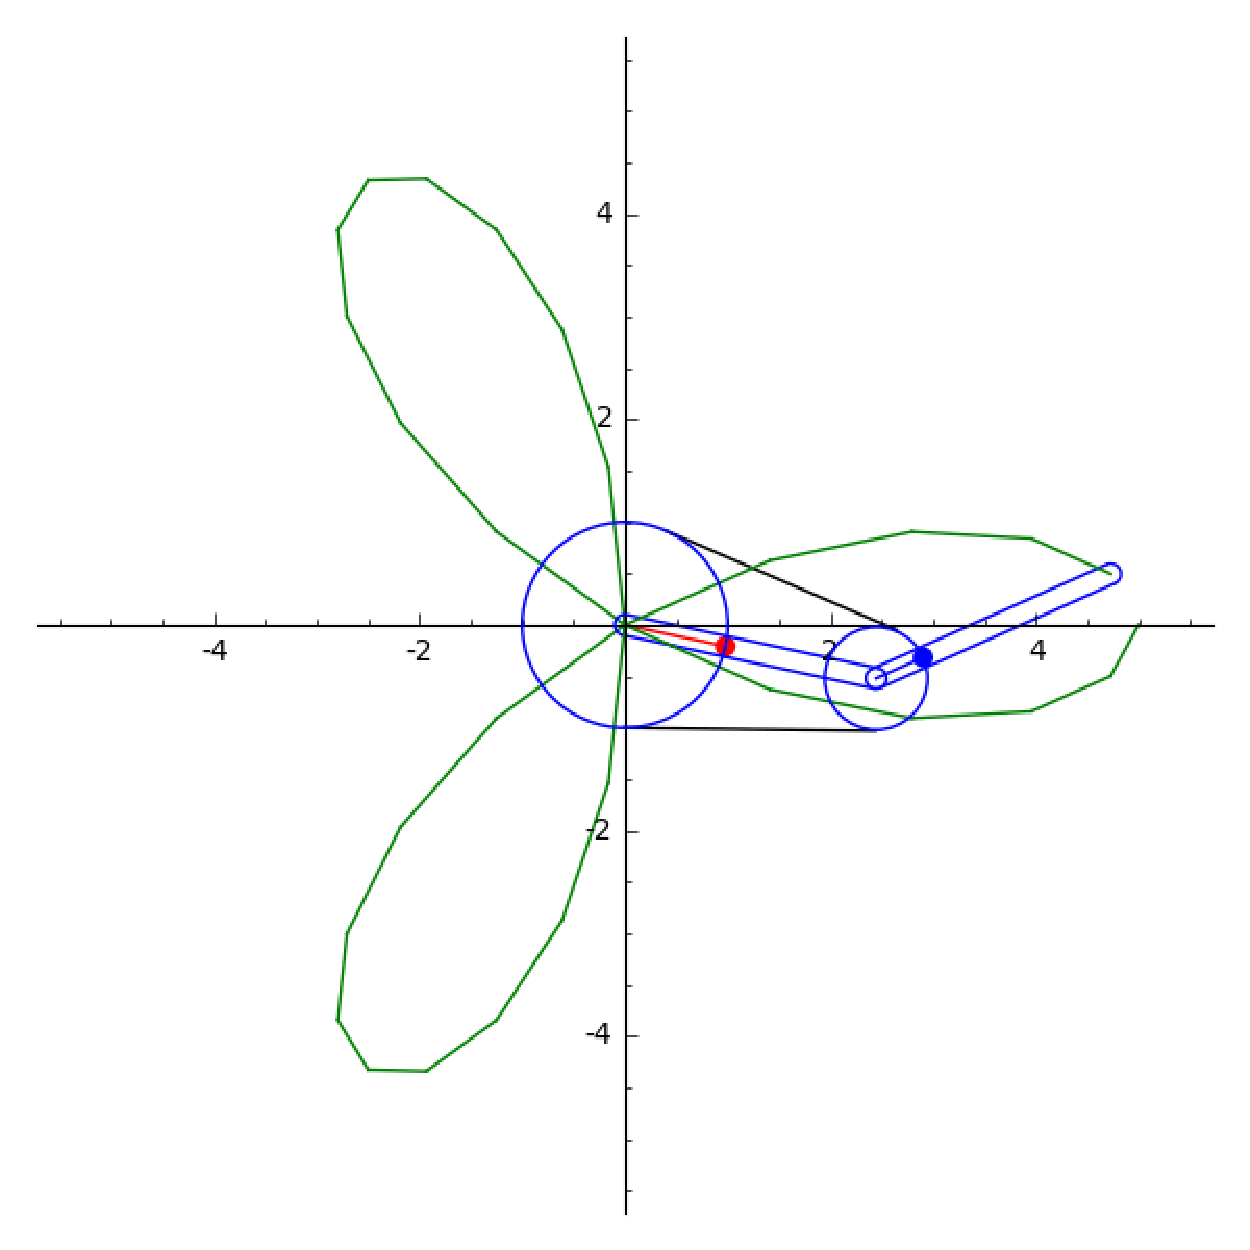
\includegraphics[width=0.3\columnwidth]{tri30.eps}
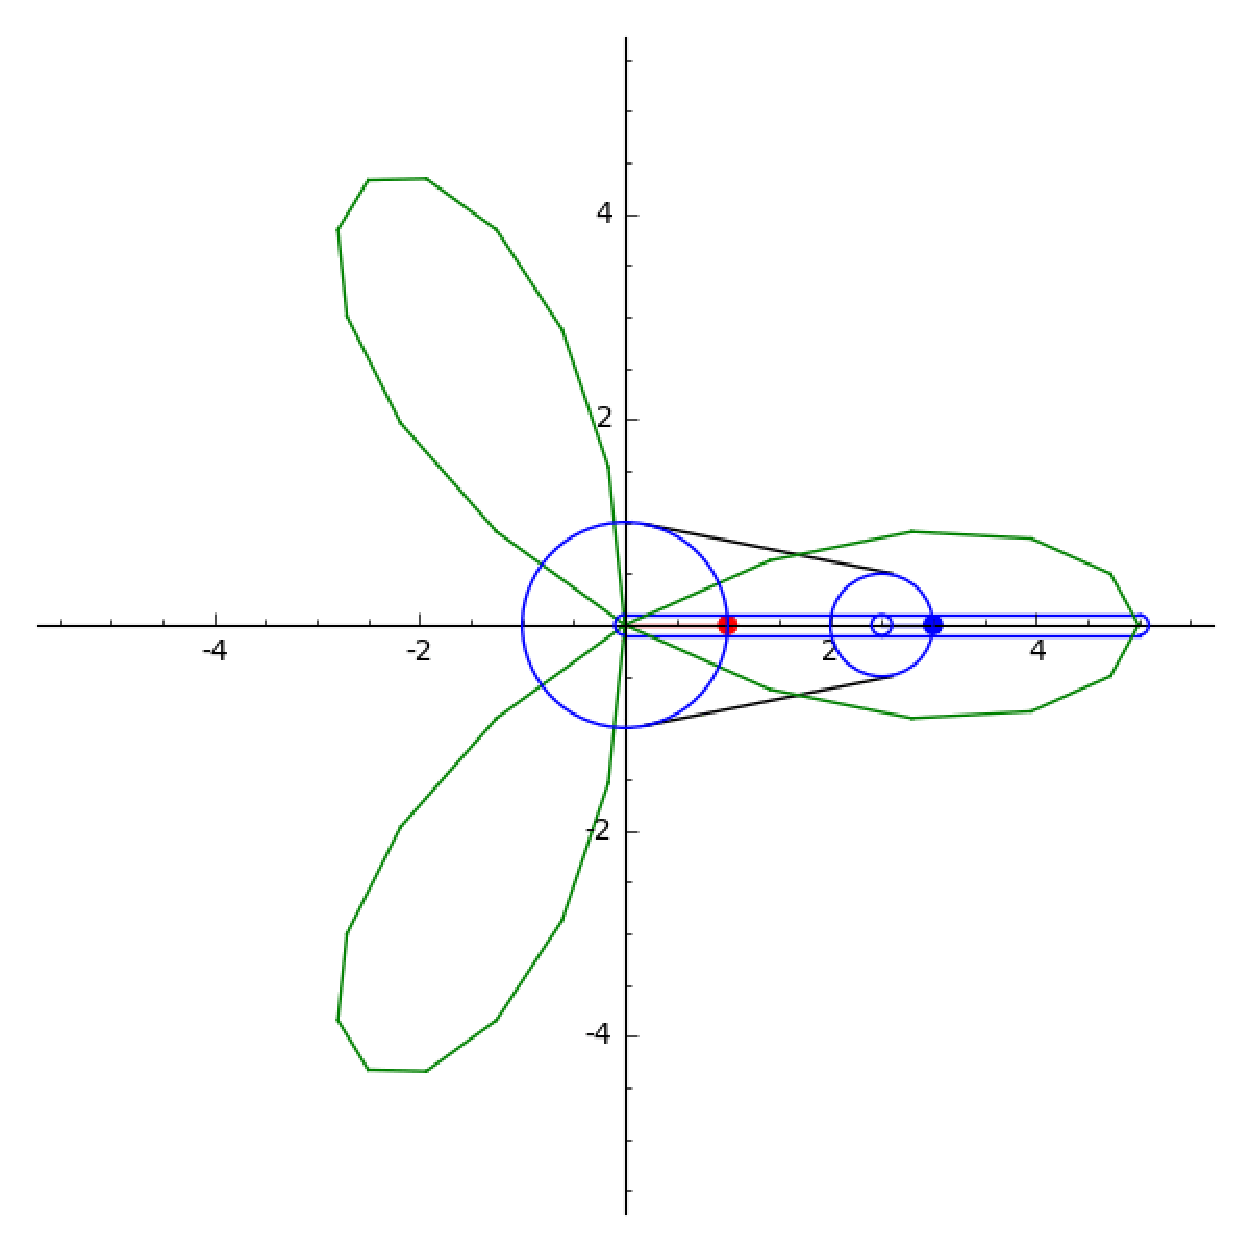
\includegraphics[width=0.3\columnwidth]{tri31.eps}\\[1em]


\end{center}

\end{block}
\end{column}%2


%-- Column 3 ---------------------------------------------------
\begin{column}{0.245\linewidth}

\begin{block}{Trigonometric Plane Curves}
A trigonometric plane curve, $P=(x(\theta),y(\theta))$, is a parameterized curve with coordinate functions that are finite Fourier series. \\

For example, this is the trigonometric plane curve equation for the trifolium:

\[
P_{T}=\begin{cases}
	\hfil -\cos{2\theta} - \cos{4\theta}\\
	\hfil \sin{2\theta} - \sin{4\theta}
	\end{cases}
\]

\end{block}


%-- Block 3-2
\begin{block}{Math}
Include math within the text is as simple as $1+1=2$. You can also
highlight more important equations like this:
$$
\int_0^1\sin(x)+\cos^2(x)+\alpha x\ dx
$$
\end{block}

%-- Block 3-3
\begin{block}{Three Pictures}
\vspace{0.5em}

\begin{center}
% THREE copies of a placeholder picture.
\includegraphics[width=0.9\columnwidth]{science}\\[1em]
\includegraphics[width=0.9\columnwidth]{science}\\[1em]
\includegraphics[width=0.9\columnwidth]{science}
\end{center}
\end{block}

%-- Block 3-4
\begin{block}{Theorems}
The beamer \texttt{theorem} environment takes up a lot of space and
adds various decorations.  Dividing the poster into blocks probably
provides enough modularity and decoration.

\vspace{1em}

Another way to typeset theorems in the poster is:

\vspace{1em}

\textbf{Theorem.}  An even perfect square is a multiple of $4$.

\vspace{0.5em}

\textbf{Corollary.}  The number $18$ is not a perfect square.
\end{block}

\end{column}%3


%-- Column 4 ---------------------------------------------------
\begin{column}{0.245\linewidth}

%-- Block 4-1
\begin{block}{Experiments}
Answer the question posed by each block heading as efficiently as
possible.  A block titled ``experiments'' should get right to the
point of explaining what experiments were conducted.
\end{block}

%-- Block 4-2
\begin{block}{Theorem}
Another option for typesetting theorems is to make the statement its
own block.
\end{block}

%-- Block 4-3
\begin{block}{Conclusions}
We find that there are infinitely many primes, and that most of them
are odd.  Also,
\begin{itemize}
\item Primes less than $n$ are slightly more likely to be quadratic
non-residues mod $p$, when $p$ is a fixed prime and $n$ is large.
\item There are infinitely many consecutive prime pairs $p_n, p_{n_1}$
satisfying $p_{n+1} - p_n < 300$.
\end{itemize}
\end{block}

%-- Block 4-4
\begin{block}{References}
\begin{thebibliography}{99}

\bibitem{design cursive}
Liu Y, Michael McCarthy JJ. Design of a Linkage System to Write in Cursive. ASME. \emph{J. Comput. Inf. Sci. Eng.} 2017;17(3):031015-031015-8. doi:10.1115/1.4037229.

\bibitem{mechanism design}
Liu Y, Michael McCarthy JJ.\emph{ Design of Mechanisms to Draw Trigonometric Plane Curves.} ASME. J. Mechanisms Robotics. 2017;9(2):024503-024503-8. doi:10.1115/1.4035882.  

\bibitem{sage}
SageMath, the Sage Mathematics Software System (Version 7.5.1),
   The Sage Developers, 2017, http://www.sagemath.org.
   
\bibitem{saxena}
Saxena, Anupam. “Kempe's Linkages and the Universality Theorem.” Resonance-Journal of Science Education, vol. 16, no. 3, Mar. 2011, pp. 220–237., www.ias.ac.in/describe/article/reso/016/03/0220-0237.

\bibitem{kempe-wiki}
Wikipedia contributors.\emph{ "Kempe's universality theorem."} Wikipedia, The Free Encyclopedia. Wikipedia, The Free Encyclopedia, 6 Sep. 2017. Web. 25 Oct. 2017.

\bibitem{synthesis of linkage}
Yang Liu, J. Michael McCarthy. \emph{ Synthesis of a linkage to draw a plane algebraic curve} "Mechanism and Machine Theory". Volume 111, 2017, Pages 10-20, ISSN 0094-114X. doi: 10.1016/j.mechmachtheory.2016.12.005.

%\bibitem{taylor-wiles} R. Taylor, A. Wiles. \emph{Ring theoretic
%  properties of certain Hecke algebras}. Ann. Math. \textbf{141}
%(1995), 553--572.
%\bibitem{wiles} A. Wiles. \emph{Modular elliptic curves and Fermat's
%  Last Theorem}. Ann. Math. \textbf{141} (1995), 443--551.
 % \bibitem{taylor-wiles}
%R. Taylor,  A. Wiles. \emph{Ring theoretic properties of certain Hecke algebras}. Ann. Math. %\textbf{141} (1995), 553--572.
%\fi
\end{thebibliography}
\end{block}
\end{column}%4

\end{columns}
\end{frame}
\end{document}
